\documentclass[utf8]{gradu3}

\usepackage{graphicx} % kuvien mukaan ottamista varten

\usepackage{amsmath} % hyödyllinen jos tekstisi sisältää matikkaa,
                     % ei pakollinen

\usepackage{booktabs} % hyvä kauniiden taulukoiden tekemiseen
\usepackage{listings}
\usepackage{color}
\usepackage{qtree}

% HUOM! Tämän tulee olla viimeinen \usepackage koko dokumentissa!
\usepackage[bookmarksopen,bookmarksnumbered,linktocpage]{hyperref}

\addbibresource{thesis.bib} % Lähdetietokannan tiedostonimi

\definecolor{light-gray}{gray}{0.96}

\lstdefinelanguage{Smalltalk}{
morekeywords={true,false,self,super,nil},
sensitive=true,
morecomment=[s][\color{blue}]{"}{"},
morestring=[d]',
alsoother={_},
style=SmalltalkStyle,
columns=fullflexible,
xleftmargin=.20in,
showspaces=false,
numbers=left,
framexleftmargin=15pt,
tabsize=4
}
\lstdefinestyle{SmalltalkStyle}{
literate={:=}{{$\gets\ $}}2{^}{{$\uparrow$}}1{_}{{$\gets\ $}}2{ä}{{\"a}}2{ö}{{\"o}}2
}

% Taken from Lena Herrmann at 
% http://lenaherrmann.net/2010/05/20/javascript-syntax-highlighting-in-the-latex-listings-package
\definecolor{lightgray}{rgb}{.9,.9,.9}
\definecolor{darkgray}{rgb}{.4,.4,.4}
\definecolor{purple}{rgb}{0.65, 0.12, 0.82}

\lstdefinelanguage{JavaScript}{
  keywords={typeof, new, true, false, catch, function, return, null, catch, switch, var, if, in, while, do, else, case, break},
  keywordstyle=\color{blue}\bfseries,
  ndkeywords={class, export, boolean, throw, implements, import, this},
  ndkeywordstyle=\color{darkgray}\bfseries,
  identifierstyle=\color{black},
  sensitive=false,
  comment=[l]{//},
  morecomment=[s]{/*}{*/},
  commentstyle=\color{purple}\ttfamily,
  stringstyle=\color{red}\ttfamily,
  morestring=[b]',
  morestring=[b]"
}

\lstset{
   language=JavaScript,
   extendedchars=true,
   basicstyle=\footnotesize\ttfamily,
   showstringspaces=false,
   showspaces=false,
   numbers=left,
   numberstyle=\footnotesize,
   numbersep=9pt,
   tabsize=2,
   breaklines=true,
   showtabs=false,
   captionpos=b
}



\begin{document}

\title{MVC-arkkitehtuurin toteutus web-sovelluskehyksissä}
\translatedtitle{Implementation of MVC-architecture in web-frameworks}
\studyline{Kaikki suuntautumisvaihtoehdot}
\avainsanat{%
  MVC,
 Web-sovelluskehys}
\keywords{MVC, Web-framework}
\tiivistelma{%
Tässä tutkielmassa esitellään MVC-arkkitehtuurin toteutusta Python-pohjaisissa web-sovelluskehyksissä. Työssä selvitetään
millä tavalla MVC on toteutettu sovelluskehyksissä ja vastaako se alkuperäistä MVC:n toteutusta. MVC:n toteutus määritellään Krasnerin artikkelissa \parencite{krasner}, joka pohjautuu Reenskaugin alkuperäiseen MVC:n määritelmään. Työssä tutkitut 
sovelluskehykset ovat Django, Pyramid ja Tornado. Django ja Pyramid eivät toteuttaneet MVC:tä. Tornadon ja web-sokettien avulla MVC on mahdollista toteuttaa.

}
\abstract{%
  This thesis goes through MVC-architecture implementation in Python-based MVC web-frameworks and answers the question if the original MVC is properly implemented. The original MVC is defined in Kranser's article \parencite{krasner} which is based on model founded by Trygve Reenskaug. The web-frameworks used thesis are Pyramid, Django and Tornado. Django and Pyramid did not implement the MVC properly. With Tornado and web-sockets the MVC-architecture is possible to implement.
uld usually say exactly the same
}

\author{Toni Haka-Risku}
\contactinformation{Ag~C416.1, \texttt{toni.haka-risku@student.jyu.fi}}
% jos useita tekijöitä, anna useampi \author-komento
\supervisor{Tommi Kärkkäinen}
\supervisor{Jonne Itkonen}
% jos useita ohjaajia, anna useampi \supervisor-komento

\maketitle

\preface
Tutkielman aiheen valintaan vaikutti aiempi kokemus ohjelmoinnista niin vapaa-ajalla kuin työelämässäkin. Suurimmassa osassa ohjelmistoprojekteja, joissa olen työskennellyt, on ollut käytössä MVC-pohjainen sovelluskehys työkaluna. Django-sovelluskehyksen sivuilla kuitenkin kyseenalaistetaan MVC:n toteutus sellaisenaan. Tästä sain idean kirjoittaa Pro Gradu tutkielman löytääkseni vastauksen kyseiseen ongelmaan. 
Jyväskylässä \today

\bigskip

Toni Haka-Risku


\begin{thetermlist}
\item[URL] Tapa nimetä objekteja ja komponentteja sovelluksessa, jolloin ne voidaan yksilöidä ja paikantaa \parencite{trends}.
\item[MVC] Model-View-Controller sovellusarkkitehtuuri.
\item[Sovelluskehys] on sovelluskehitykselle tarkoitettu pohja, joka kutsuu käyttäjän kirjoittamaa ohjelmakoodia ja tarjoaa ratkaisuja yleisimpiin toistuviin ongelmiin
\item[WSGI] Määrittää miten web-palvelin kommunikoi web-sovellusten kanssa ja millä tavalla web-sovellukset yhdistetään prosessoimaan pyyntöjä.
\item[Template] Dynaaminen HTML-pohja, johon voidaan kirjoittaa ohjelmalogiikkaa
\item[Pakettikytkentä] Tiedonsiirtomenetelmä, jossa data jaetaan paketeiksi. Osapuolien väliseen viestintään ei varata kaistaa, eikä osapuolien välille luoda katkeamatonta yhteyttä \parencite{kytkenta}.
\item[Piirikytkentä] Tiedonsiirtomenetelmä, jossa yhteys pysyy auki riippumatta siitä, onko osapuolien välillä liikennettä. Piirikytkentä on käytössä esim. puhelinverkoissa \parencite{kytkenta}.
\item[Asiakas] Alustaa yhteyden lähettääkseen pyyntöjä palvelimelle \parencite{http}.
\item[HTTP] Yksisuuntainen kommunikaatio-protokolla hypertekstidokumenttejen siirtoon. Määrittelee kahdeksan perusoperaatiota: OPTIONS, GET, HEAD, POST, PUT, DELETE, TRACE ja CONNECT. Käytetyimmät operaatiot ovat GET ja POST. 
\item[Käyttäjä-agentti] on tietokoneohjelma, joka lähettää pyynnön jollekin tietylle ohjelmalle. Tällaisia ovat esimerkiksi selaimet \parencite{http}. 
\item[Palvelin] Tietokoneohjelma, joka ottaa vastaan yhteyksiä ja lähettää takaisin vastauksia asiakassovellukselle. Jokainen ohjelma pystyy olemaan yhtäaikaa asiakassovellus ja palvelin \parencite{http}. 
\item[Web-soketti] TCP:n päällä toimiva protokolla, joka mahdolllistaa kaksisuuntaisen kommunikaation asiakkaan ja palvelimen välillä \parencite{websocket}.
\item[TCP] Protokolla kahden isännän väliseen luotettavaan tiedonsiirtoon verkossa  \parencite{tcp1_1}.
\end{thetermlist}

\mainmatter

\chapter{Johdanto}

1994-luvulla Internet tuli julkisesti kaikkien saataville ja tämän jälkeen siitä on tullut alusta lukuisille web-sovelluksille. Web:n ensimmäiset toteutukset koostuivat suurista määristä dokumentteja, joita pystyttiin
yhdistämään toisiinsa hyperlinkeillä. Nämä olivat usein yksinkertaisia tekstitiedostoja, joissa sisältö oli staattista. Yhdessä vuosikymmenessä Web on kuitenkin muuttunut staattisesta arkistosta kattavaksi alustaksi sovellusten toteuttamiseen ja julkaisuun. Uudet web-teknologiat, metodit ja kielet mahdollistavat dynaamisten sovellusten luonnin sekä mallintamisen käyttäjien välille. Web-sovelluksissa tullaan kehittymään sitä mukaan, kun uusia teknologioita otetaan käyttöön web-selaimissa \parencite{trends}. 

Web:n arkkitehtuurissa palvelin tarjoaa asiakassovellukselle web-sivuja, jotka voidaan dynaamisesti luoda palvelimen ohjelmakoodin avulla. Esimerkiksi selaimen pyytäessä web-sivua, tehdään pyyntö palvelimelle. Pyynnön perusteella palvelin hakee tietokannasta tarvittavat tiedot ja muodostaa niistä sivun, joka palautetaan vastauksena takaisin selaimelle. Palvelimen puolella toteutettu sivujen prosessointi johti CGI-sovelluksiin (Common Gateway Interface), missä sovelluksen yksittäinen URL yhdistetään ohjelmakoodiin. Sovelluksen kasvaessa ohjelmakoodin hallinta osoittautuu kuitenkin vaikeaksi monien dynaamisten sivujen generoinnin osalta. Tämän ongelman ratkaisemiseksi kehittyi hybridimalli, jossa ohjelmakoodin palasia kirjoitetaan esimerkiksi HTML:n sekaan, jolloin halutut osat voidaan muuttaa dynaamiseksi. Pyynnön aikana dynaamiset ohjelmakoodin palaset suoritetaan ja yhdistetään dokumenttiin. PHP-ohjelmointikielellä oli tähän merkittävä vaikutus. Ratkaisu teki sivujen uudelleenkäyttämisen helpommaksi, mutta ajan kuluessa huomattiin koodimuutoksien olevan vaikeasti toteutettavissa, kun ohjelmakoodin palaset olivat käytössä kaikkialla sivuilla. Tämä puolestaan johti lopulta malliin, jossa sovelluksen tietty osa hallitsee pääsyä dataan ja toinen osa hajotetaan palasiin, joilla hallitaan sivujen luontia ja käyttäjien näkymiä \parencite[3.1]{trends}

Tyypillinen rakenne web-sovelluksissa koostuu seuraavista osista: 
\begin{itemize}
\item HTML-sivujen näyttäminen käyttäjälle.
\item Selaimen puolella ajettava ohjelmakoodi.
\item Palvelimen puolella ajettavat ohjelmakoodi, jotka tyypillisesti keskustelevat tietokantojen kanssa.
\end{itemize}

Selaimessa käytetty ohjelmointikieli perustuu ECMAScript-standardiin, joka on olio-pohjainen ohjelmointikieli ja erityisesti tarkoitettu käyttöön selaimen puolelle. Tunnetuin ECMAScriptin toteutus on JavaScript. Palvelimen puolella ohjelmointikieliä on useita. Tällaisia ovat esimerkiksi PERL, PHP, Python ja Ruby. Palvelinpuolen ohjelmointikielien pohjalta on luotu lukuisia sovelluskehyksiä, joissa pohjana on käytetty MVC-arkkitehtuuria. Näistä tunnetuimpia ovat Ruby-kielellä toteutettu Ruby On Rails sekä Pythonilla toteutettu Django \parencite{trends}. Tässä tutkielmassa käydään Pythonilla toteutettu Pyramid-sovelluskehyksen MVC-arkkitehtuurin rakenne läpi ja heijastetaan toteutusta alkuperäiseen MVC:n määritelmään. Lisäksi käydään lyhyesti läpi Djangon toteutus, joka on hyvin lähellä Pyramidin toteutusta. Lopuksi toteutetaan MVC-arkkitehtuuri itse käyttäen pohjana Tornado-sovelluskehystä.

\section{Tutkimuskysymys}
Tutkimuksen tarkoituksena on selvittää ohjelmistokehityksen ja ohjelmistoarkkitehtuurejen taustoja. Lisäksi käydään läpi tärkeimmät web-teknologiat, joiden päälle Internet on rakennettu. Näiden pohjalta tutkitaan millä tavalla 
Model-View-Controller -arkkitehtuuri (MVC) on toteutettu web-sovelluskehyksissä ja miten se
eroaa alkuperäisestä arkkitehtuurin määritelmästä, jonka määrittelee Krasner \parencite{krasner} käyttäen pohjana Reenskaugin kehittelemää MVC-arkkitehtuuria \parencite{reenskaug_tools}. Web-sovelluskehyksen voidaan sanoa toteuttavan MVC-arkkitehtuuri, kun sen komponentit pystytään jaottelemaan määritelmän mukaisesti Malliin (Model), Näkymään (View) ja Ohjaimeen (Controller) siten, että ne toteuttavat määritelmän mukaiset roolit. Malli hallitsee sovelluksen tilaa, Ohjain ottaa vastaan syötteitä ja Näkymä huolehtii käyttöliittymän piirtämisestä käyttäjälle. Mallin tulee pystyä lähettämään sekä vastaanottamaan viestejä Ohjaimelta ja Näkymältä. Ohjaimen tulee pystyä lähettämään viestejä näkymälle. MVC-pohjaisten web-sovelluskehyksien tutkimisen jälkeen pyritään toteuttamaan MVC alkuperäisen määritelmän mukaan Tornado-sovelluskehyksellä käyttäen TCP-protokollan päällä toimivaa Web-soketti protokollaa kommunikaatiossa HTTP:n sijaan. Havaintojen pohjalta selvitetään voidaanko Reenskaugin ja Krasnerin määrittelemä MVC-arkkitehtuuri toteuttaa web-sovelluskehyksellä. 

\section{Tutkimuksen rakenne ja aiheen rajaus}
Tutkimuksessa käytetään laadullista tutkimusmenetelmää. Hypoteesi on kuitenkin vahvasti läsnä tutkielman aikana, koska tutkielma perustuu olettamukseen MVC:n toteutuksesta web-sovelluskehyksissä. Tutkimus ei todista mitään MVC:n aihealueen ulkopuolelta vaan pyrkii esittämään yleisiä oletuksia 
MVC:n suhteesta web-sovellusten toteutuksiin sovelluskehyksien avulla. Tutkimuksen päämääränä on joko vahvistaa tai kumota hypoteesi MVC:n soveltuvuudesta web-sovelluskehyksillä toteutettuihin web-sovelluksiin. 

Internettiä ja WWW:tä (World Wide Web) varten toteutetuissa web-sovelluksissa toistuvat usein samat toiminnallisuudet, kuten esimerkiksi staattisten resurssejen jakaminen, URL:ien liittäminen ohjelmakoodiin sekä tietoturvan hallinta \parencite{pyramid_intr}. Tällöin on tärkeää, että Internetin ja WWW:n taustat käydään tutkielmassa läpi, sillä niiden merkitys on suuri web-sovelluskehyksien olemassaololle. HTTP-protokollalla on myös suuri rooli MVC:n suhteen, koska se on pohjimmiltaan tarkoitettu yksisuuntaiseen viestintään, vaikka MVC:n alkuperäisenä ajatuksena on kaksisuuntainen kommunikaatio esimerkiksi Mallin ja Näkymän välillä \parencite{reenskaug_tools}. HTTP:n lisäksi käydään läpi Internet Protokollan, TCP:n sekä Web-soketin toteutukset läpi. Web-soketti protokollalla pyritään ratkaisemaan kaksisuuntaisen kommunikaation ongelma MVC:ssä.

Tutkimus aloitetaan kirjallisuuskatsauksella, jossa tarkastellaan mitä aiempaa 
tutkimusta ohjelmistokehityksestä ja MVC:stä on tehty. Lisäksi käydään
läpi mitä lähteitä löytyy Python-pohjaisista web-sovelluskehyksistä sekä ohjelmistoarkkitehtuureista. Web-sovelluskehykset rajataan 
Pyramid-, Django- ja Tornado-sovelluskehyksiin. Tämän jälkeen tutkitaan Internetin ja WWW:n taustoja sekä avataan ohjelmistoarkkitehtuurejen merkitystä tutkielmalle. Seuraavaksi käydään läpi MVC:n historiaa sekä millä tavalla MVC on tarkoitettu toteutettavaksi. Tässä vaiheessa esitellään jokaisen MVC-komponentin tarkoitus sekä niiden 
keskinäisen kommunikaation rakentuminen. Lisäksi esitellään
Dortmundin yliopistossa kirjoitettu esimerkkiohjelma Smalltalk-ohjelmointikielellä siitä miten MVC:n 
toteutus tuodaan sovellukseen käytännössä.

MVC:n tarkastelun jälkeen esitellään tutkielmassa käytetyt web-sovelluskehykset, 
joita käytetään apuna MVC:n tutkimisessa. MVC:stä on olemassa erilaisia versioita, joten sen määrittely tulee rajata tarkasti.
Kun puhutaan MVC:stä, tarkoitetaan tällä Krasnerin artikkelissa esiteltyjä määrittelyitä MVC:n toteutuksesta \parencite{krasner}, jotka pohjautuvat Trygve Reenskaugin esittelemään 
MVC:n määritelmään \parencite{xerox-original}. 

Tarkasteltavista sovelluskehyksistä Pyramid ja Django ovat MVC-arkkitehtuuriin pohjautuvia sovelluskehyksiä. Tornado on asynkroninen sovelluskehys, jota käytetään tutkielmassa toteuttamaan MVC alkuperäisen toteutuksen mukaisesti käyttäen web-soketteja. Sovelluskehyksistä käydään läpi sen 
historia sekä yleisellä tasolla mihin käyttötarkoitukseen
sovelluskehys on tarkoitettu. Tämän jälkeen verrataan MVC:n toteutusta 
Pyramid- ja Django-sovelluskehykseen ja selvitetään, millä tavalla näiden sovellusarkkitehtuuri mahdollisesti eroaa MVC:n alkuperäisestä toteutuksesta. Sovelluskehyksien muihin teknisiin ominaisuuksiin ei oteta kantaa.
Havaintojen perusteella pohditaan MVC:n mahdollisia ongelmia sovelluskehyksien toteutuksessa 
ja selvitetään löytyykö sovelluskehyksien arkkitehtuurista jotain yhtenäisiä piirteitä, mitkä ovat
kytköksissä MVC:n toteutukseen. Saatujen tulosten pohjalta pyritään kirjoittamaan Tornado-sovellus, joka toteuttaa MVC:n 
alkuperäisen määritelmän mukaan. Tutkimuksen lopuksi koostetaan havainnoista yhteenveto, jossa pohditaan saatuja tuloksia ja selvitetään 
pystytäänkö niiden perusteella vastaamaan tutkimuskysymykseen.


\pagebreak
\section{MVC:n ongelmat web-kehityksessä}
Sovellusarkkitehtuurin tarkoituksena on vastata millä tavalla ohjelmiston eri komponentit ovat organisoitu, rakennettu ja millä tavalla ne kommunikoivat keskenään. Tämä on ensimmäinen vaihe, kun ohjelmistoa lähdetään toteuttamaan. MVC on yksi tapa
toteuttaa sovelluksen arkkitehtuuri \parencite[s. 148]{Sommerville}. MVC-arkkitehtuuri on saanut paljon huomiota web-sovelluskehyksien
toteutuksissa ja useat web-sovelluskehykset ovat luokiteltu
MVC-sovelluskehyksiksi \parencite{mvcframeworks}. Tätä tukee myös Sommervillen teos, jossa väitetään web-sovelluskehysten olevan suurimmaksi osaksi MVC-arkkitehtuurin toteuttavia \parencite[s. 432]{Sommerville}.
Se on kuitenkin alunperin tarkoitettu matalan tason käyttöliittymäsovellusten toteuttamiseen,
jossa esimerkiksi hallitaan yksittäisiä näppäimistöltä tulleita
syötteitä eikä sitä ole suoraan tarkoitettu käytettäväksi
web-sovellusten ohjelmointiin. Alkuperäisen MVC:n toteutuksen
soveltuvuutta web-ohjelmointiin onkin epäilty. Esimerkiksi Leff
soveltaa artikkelissaan MVC:n käyttämistä web-sovelluksissa, mutta
samalla esittelee alkuperäisen MVC:n toteuttamisen ongelmana. Tämä johtuu web-sovelluksen jakautumisesta asiakkaan
(client) ja palvelimen (server) välille \parencite{ibm_watson}. Myös Pyramid-sovelluskehyksen tekijät
kyseenalaistavat MVC-arkkitehtuurin toteutuksen Pyramidissa ja uskovat
MVC:n olevan sellaisenaan sopimaton web-ohjelmointiin, vaikka
Pyramidin toteutus onkin hyvin lähellä alkuperäistä MVC:tä
\parencite{pyramid}. Django on vastaavasti toteutettu MVC:n pohjalta, mutta sen väitetään toteuttavan MVC eri tavalla, kuin MVC:n määritelmässä \parencite{django_mvc}.
Sommerville \parencite[s. 157]{Sommerville} esittelee MVC:n yhtenä arkkitehtuurimallina, jonka hän luokittelee
kerrosarkkitehtuurien (Layered architecture) joukkoon. Sommervillen esittelemä MVC-malli kuitenkin poikkeaa Krasnerin \parencite{krasner} määrittelemästä MVC-mallista. Alla esitetään Krasnerin määrittelemä MVC-malli sekä Sommervillen määrittelemä MVC-malli:
\pagebreak

\begin{figure}[h]
\centering
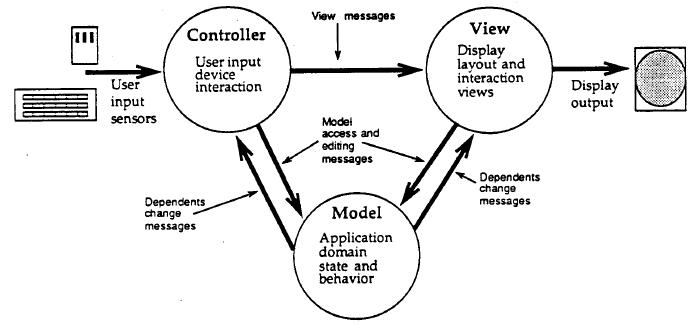
\includegraphics[scale=0.5]{krasner_mvc.jpg}
\caption{\parencite[s. 5]{krasner_desc}}
\end{figure}

\begin{figure}[h]
\centering
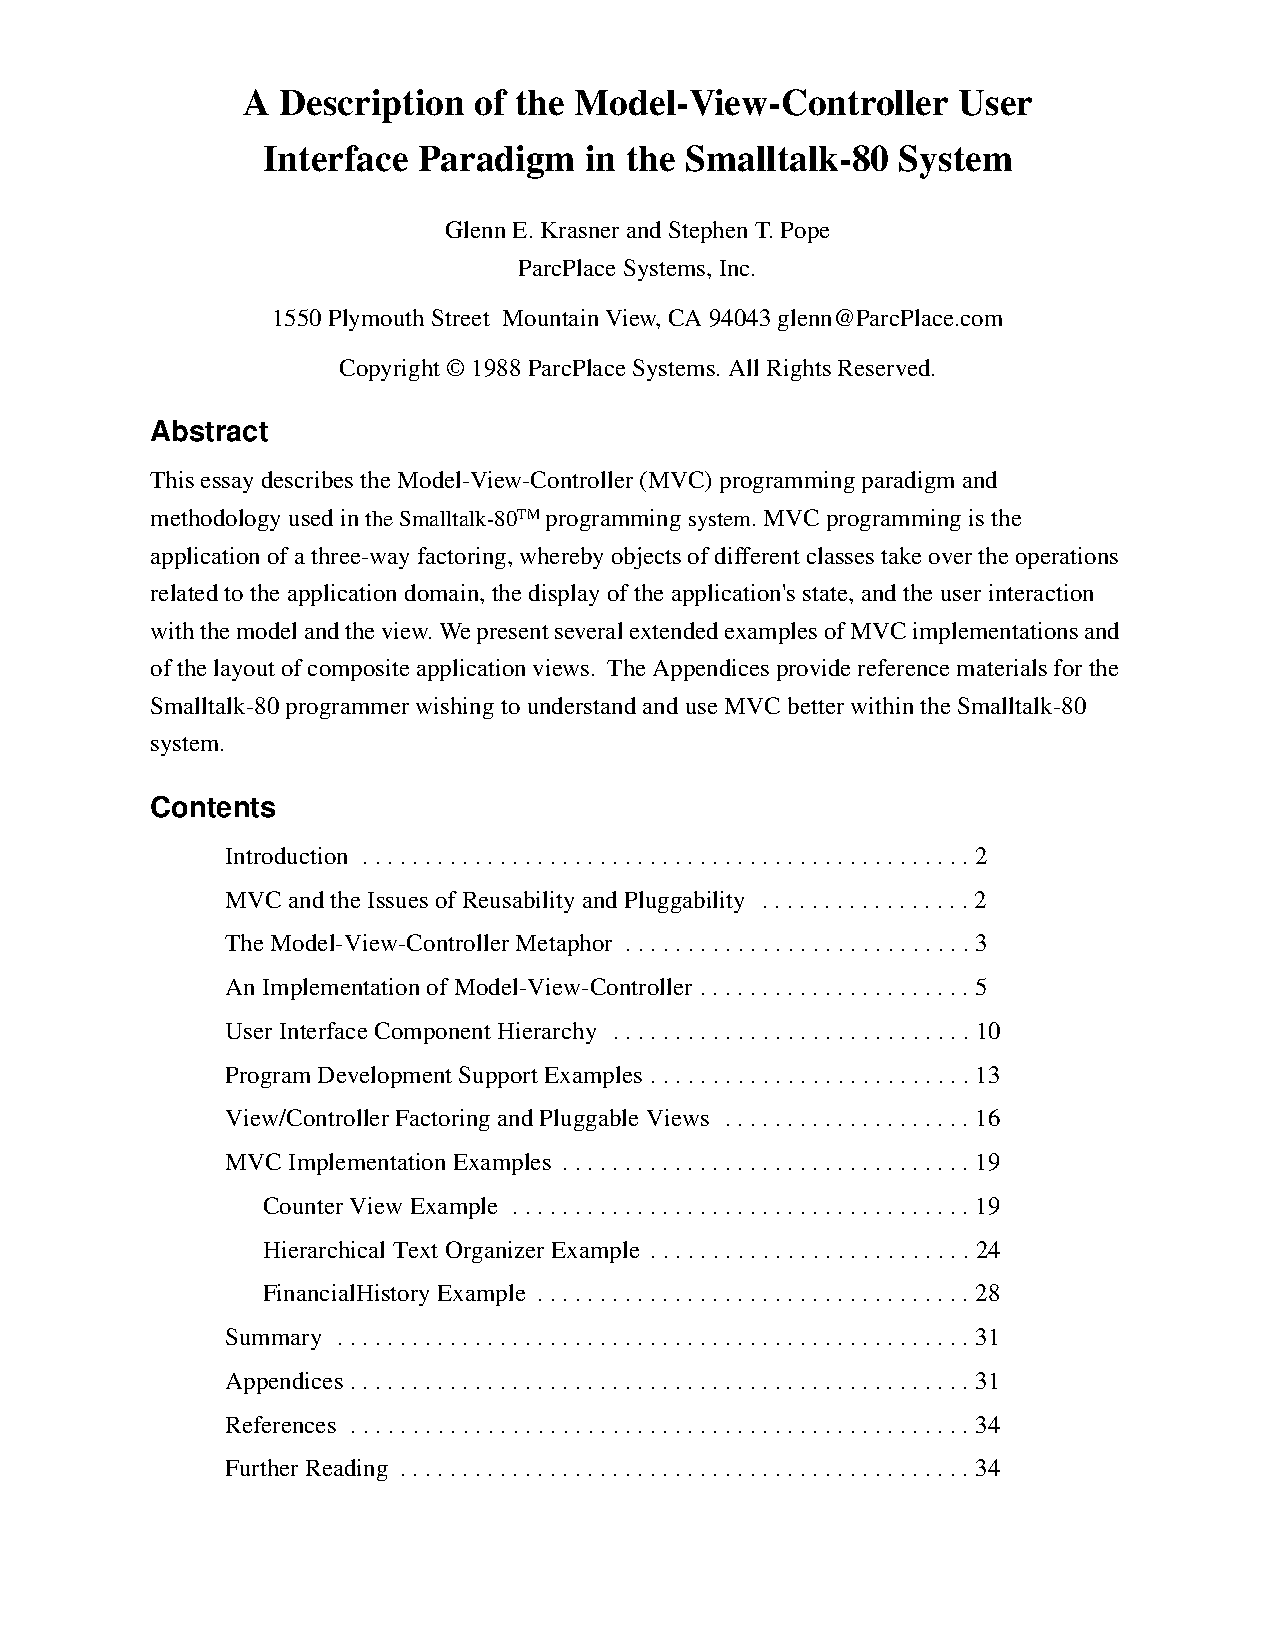
\includegraphics[scale=0.45]{mvc.png}
\caption{\parencite[s.162]{Sommerville}}
\end{figure}


Krasnerin esittelemässä MVC:ssä Malliin (Model) on rekisteröity Ohjaimia (Controller) ja Näkymiä (View). Näin Malli pystyy kommunikoimaan muutoksistaan suoraan Ohjaimelle sekä Näkymälle.
Sommerville esittelee MVC-mallin web-sovelluksen näkökulmasta, jossa kommunikointi komponettejen suhteen toteutetaan erilailla. Sommervillen mallissa tieto käyttäjän toiminnoista voi tulla 
Näkymältä. Käyttäjän pyynnöt voivat tulla niin Ohjaimelle kuin Näkymällekin toisin kuin Krasnerin mallissa, jossa käyttäjän toiminnot tulevat ainoastaan Ohjaimelle.
Lisäksi Sommervillen määritelmässä Mallilla ei ole kaksisuuntaista yhteyttä Ohjaimeen. 

Kuten nähdään, MVC-arkkitehtuurin toteutukset poikkeavat toisistaan ja sen määritelmä on vuosien saatossa muuttunut erityisesti web-kehityksen myötä. Tästä syystä MVC:stä on monenlaisia toteutuksia. Erityisesti komponenttejen kommunikaatio poikkeaa eri toteutusten välillä. 
\chapter{Lyhyt kirjallisuuskatsaus}

Kirjallisuuskatsauksessa käydään läpi, millä tavalla lähdemateriaalia kerätään tutkielmaa varten. Lähdemateriaalin 
haku toteutetaan hakukoneilla, jotka ovat tarkoitettu erityisesti 
tieteellisten artikkeleiden etsimiseen. Tässä tutkielmassa käytetyt 
hakukoneet ovat seuraavat: IEEE Xplore, ACM Digital Library, 
Google Scholar sekä joissakin tapauksissa Google:n yleinen
hakukone. Yleistä hakukonetta on käytetty esimerkiksi
sovelluskehyksien dokumentaatioiden etsintään.

Aluksi muodostetaan kokonaiskuva tuloksista, jossa silmäillään läpi
saatuja artikkeleita. Tässä vaiheessa tarkoitus ei ole vielä valita
mitään pohjaksi tutkielmalle, vaan kerätä informaatiota siitä
millainen lähdemateriaali on tarjolla kokonaisuudessaan. Saaduista 
tuloksista poimitaan artikkeleita, jotka sopivat tutkielman aihepiiriin.
Seuraavaksi artikkeleista valitaan tutkielmalle
pohjakirjallisuus. Artikkelit luetaan huolellisesti
läpi ja varmistutaan siitä, että ne ovat tieteellisesti päteviä
tutkielmaa varten. Erityisesti kiinnitetään huomiota viittauksien
määrän valittaessa tärkeimmät lähdemateriaalit. Tutkielmassa esiintyy myös satunnaisia viittauksia,
joita ei ole kirjallisuuskatsauksessa mainittu. Tutkimuksen
pääkirjallisuus kuitenkin käydään läpi kirjallisuuskatsauksessa.
Haussa käytetään seuraavia hakutermejä: "software engineering", "software development", "MVC", "MVC Architecture",
"frameworks", "web-frameworks" ja "websocket". Alla esitellyssä taulukossa näytetään hakujen tuottamien tulosten määrä, jossa hakukriteerinä käytetty
metatietoja sekä otsikkoa.


\begin{center}
\begin{tabular}[t]{|p{120pt}|p{90pt}|p{90pt}|p{90pt}|p{90pt}|}
    \hline
    Hakusana  & ACM digital library & IEEE Xplore & Google Scholar\\
    \hline
    "software engineering"   & 3 639    & 4 971 & 55 500  \\
    "software development" & 21 729  & 3,045 & 60 900 \\
    "MVC"  			 &  20	       & 1 068 & 5 320  \\
    "MVC architecture"          &  49        & 308 & 122 \\
   "frameworks" 		 &  44 824 & 174 731 & 79 700 \\
   "web-frameworks" 	 &  7 848   & 50 & 136 \\
   "websocket"                     & 37        &   934 000 &  9 340 \\
    \hline
\end{tabular}
\end{center}

\section{Sovelluskehitys ja arkkitehtuurit}
Sovelluskehityksen tarkasteluun löytyy runsaasti lähdemateriaalia. Merkittäväksi lähteeksi valitaan Ian Sommervillen julkaisema \textit{Software Engineering 9th Edition} -kirja, jossa käydään läpi mitä asioita suurien ohjelmistojen kehittämiseen kuuluu \parencite{Sommerville}. Kirja on jaettu neljään pääosioon: \textit{Introduction to Software Engineering}, \textit{Dependability and Security}, \textit{Advanced Software Engineering} ja \textit{Software Management}. Tutkimuksessa lähteenä käytetään \textit{Introduction to Software Engineering} ja \textit{Advanced Software Engineering} -osioita. \textit{Introduction to Software engineering} käy läpi ohjelmistojen suunnittelua ja toteutusta yleisesti. Tällaisia ovat esimerkiksi vaatimusmäärittelyt, prosessit, arkkitehtuuri ja testaus. \textit{Advanced Software Engineering} esittelee ohjelmistojen kirjoittamista siten, että ne olisivat mahdollisimman uudelleen käytettäviä ja ylläpidettäviä. Tähän tarjotaan ratkaisuksi erilaisia sovellusarkkitehtuureja, kuten esimerkiksi \textit{Component-based architecture} ja \textit{Service-oriented architecture} \parencite{Sommerville}.

\section{MVC}
Google Scholarin tuloksista löytyy kolme artikkelia MVC:stä, jotka sopivat 
lähdemateriaaliksi tutkielmaan. Ensimmäinen artikkeleista on John
Deaconin kirjoittama artikkeli, joka tarkastelee lyhyesti
MVC:tä \parencite{deacon}. Artikkeli on kuitenkin hyvin suppea, mutta selittää
tiivistetysti MVC:n idean. Toinen artikkeli on Steve Burbeckin kirjoittama, 
joka käsittelee
MVC:tä sellaisena kuin sitä käytettiin Smalltalkissa \parencite{burbeck}. Burbeckin
artikkeliin viitataan monissa MVC:tä käsittelevissä
julkaisuissa, joten sen arvo tämän tutkielman pohjakirjallisuudessa on
vahva. Viittausten määrä on katsottu hakemalla artikkelia Google
Scholarin hakukoneessa. Seuraavaksi kartoitetaan pohjakirjallisuutta käyttäen ACM Digital
Library sekä IEEE XPlore -hakukoneita. Kolmas artikkeli Glenn
E. Krasnerin kirjoittama julkaisu, jossa esitellään MVC:n toteutusta
erilaisissa Smalltalk-sovelluksissa. Julkaisusta löytyy useita
versioita, joista käytetään
molempia \parencite{krasner} \parencite{krasner_desc}. Tähän artikkeliin on
myös viitattu runsaasti, joten se on Burbeckin julkaisun kanssa
tärkeimpiä lähteitä MVC:n pohjakirjallisuudessa. Kirjoitushetkellä
viittauksia Krasnerin artikkeliin on 2263. Monien MVC-arkkitehtuuria soveltavien artikkeleiden
lähdeviitteistä löytyy viittauksia Burbeckin ja Krasnerin
artikkeleihin. Tämän perusteella pystytään toteamaan kyseisten
artikkeleiden olevan tieteellisesti päteviä ja tarjoavan kattavan
lähdemateriaalin MVC:n pohjaksi. Burbeckin ja Krasnerin kirjoittamien
artikkeleiden taustalta löytyy MVC-arkkitehtuurin alkuperäinen kehittäjä Trygve
Reenskaug, jonka omia julkaisuja sekä kotisivujen MVC-osiota käytetään 
lähteenä tutkielmassa \parencite{xerox}.

\section{Web-sovelluskehykset \& Internet}
Internetin taustojen selvitykseen käytetään IETF:n (The Internet Engineering Task Force) dokumentaatioita \parencite{ietf}. Dokumentaatiota käytetään TCP:n, Internet Protokollan, HTTP:n ja Web-soketin taustojen selvittämiseen. Yksittäisistä web-sovelluskehyksistä löydetty kirjallisuus on hyvin
suppea, eikä tämän varaan voida rakentaa kovinkaan perusteellista
tieteellistä pohjaa. Tämän vuoksi tutkielmassa käytetään
sovelluskehyksien omia dokumentaatioita lähdemateriaalina. IEEE Xploren ja ACM Digital Libraryn avulla löytyy kaksi julkaisua, 
joita käytetään tutkielman pohjana sovelluskehyksiä
tarkastellessa. Ensimmäinen artikkeli on Okanovicin ja Mateljan
kirjoittama artikkeli, jossa esitellään web-sovelluskehyksien suunnittelua \parencite{ockanovic}. 
Se myös sivuuttaa lyhyesti MVC:tä. Toisena artikkelina käytetään ACM:n hakutuloksena saatua Iwan
Vosloon julkaisua, jossa käydään läpi yleisesti web-sovelluskehyksien
rakennetta \parencite{vosloo}. Lisäksi käytetään
IEEE:stä Ahamedin julkaisua, jossa esitellään sovelluskehyksen valintaan liittyviä asioita \parencite{towards_framework}.

Web-soketin lähdemateriaalina käytetään IETF:n dokumentaatiota \parencite{websocket} sekä Google Scholarin hakutuloksista löydettyä artikkelia, jossa toteutetaan reaaliaikainen monitorointisovellus käyttäen Web-soketteja \parencite{websocket_ajax}. Tornado-sovelluskehyksestä löytynyt materiaali on hyvin suppeaa, jolloin käytetään Tornadon omia dokumentaatioita. Tarkemmin käydään läpi Tornadon tarjoamat teknologiat, jotka ovat keskeisessä roolissa MVC:n toteutuksen selvittämisessä. Näistä tärkeimpänä Web-soketti -teknologia.

\chapter{Sovelluskehitys}
Katsomalla ympärille nykyajan yhteiskunnassa, huomataan monien asioiden toimivan ohjelmien varassa. Puhelimet, elektroniset kellot, autot ja erilaiset yhteiskunnalliset palvelut sisältävät kaikki ohjelman, jolla toimintoja sekä dataa hallitaan. Nykyajan modernia yhteiskuntaa ei pystytä ylläpitämään ilman sovelluksia. Monet tuotantolinjastot sekä rahoitusjärjestelmät teollisuudessa ovat täysin automatisoituja. Viihdeteollisuus kuten musiikki, pelit, elokuvat ja televisio ovat kaikki monimutkaisten sovellusten varassa. Ihmisten tiedot ovat monissa valtion hallintajärjestelmissä sekä niin julkisissa kuin yksityisissäkin potilastietojärjestelmissä. Useiden tavallisten arkisten asioiden taustalla on ohjelma. Suuri määrä ihmisiä kirjoittaa sovelluksia nykypäivänä. Liike-elämässä ihmiset kirjoittavat taulukkolaskentaohjelmia helpottaakseen työtään. Tutkijat ja insinöörit kirjoittavat ohjelmia prosessoimaan kerättyä dataa ja harrastelijat kirjoittavat ohjelmia viihdyttääkseen itseään. Suurin osa sovelluskehityksestä on kuitenkin toteutettu ammattilaisten toimesta tukemaan liiketoimintamalleja, kehittämään laitteita sekä rakentamaan erilaisia palveluita. Ammattilaisten toteuttamat ohjelmistot toteutetaan usein ryhmissä ja ne ovat suunnattu käytettäväksi muille kuin ohjelmoijille itselleen \parencite[s.4]{Sommerville}.

Sovelluskehityksellä tarkoitetaan koko ohjelmiston elinkaaren mittaista tuotantoprosessia alkumäärittelyistä ylläpitoon asti. Se on ammattihaara, joka on erikoistunut tutkimaan ja tuottamaan sovelluksia. Sovelluskehittäjät käyttävät erilaisia teorioita, käytänteitä ja työkaluja ratkaisemaan sovelluskehitykseen liittyviä ongelmia. Sovelluskehitys ei kuitenkaan keskity ainoastaan teknisiin ongelmiin vaan myös projektin hallintaan ja työkaluihin, jotka tukevat sovellusten kehittämistä \parencite[s.1-10]{Sommerville}. 

\section{Sovellukset}
Ohjelmistot ovat abstrakteja ja aineettomia. Ne eivät noudata mitään fysiikan lakeja eivätkä ne koostu mistään materiasta tai tuotantoprosessista. Tämä tekee ohjelmistokehityksestä vapaata, koska sille ei ole asetettu mitään luonnollisia esteitä. Rajojen puuttuminen johtaa myös siihen, että ne voivat olla usein erittäin monimutkaisia, vaikeita ymmärtää ja kallista muuttaa. Ohjelmistojen tyypit vaihtelevat sulautetuista järjestelmistä maailmanlaajuisiin tietojärjestelmiin. Tietojärjestelmän kehittäminen organisaatiolle eroaa täysin esimerkiksi ohjainlaitteen ohjelmoinnista. Näitä kahta taas ei voi verrata esimerkiksi grafiikkapohjaiseen pelikehitykseen. Kuitenkin kaikki nämä tarvitsevat ohjelmistokehitystä \parencite[s.1-10]{Sommerville}. Ohjelmistot eivät ole pelkästään tietokoneohjelmia vaan ne koostuvat ohjelman lisäksi dokumentaatioista sekä erilaisista konfiguraatioista, joilla määritellään ohjelma toimimaan tietyllä tavalla. Dokumentaatio sisältää usein tiedon ohjelmiston rakenteesta sekä käyttäjille suunnatun ohjeen miten sovellusta hallitaan ja käytetään \parencite[s.1-10]{Sommerville}. 

Sommerville jakaa ammatilaisten kehittämät ohjelmistotuotteet kahteen kategoriaan: geneeriset tuotteet ja räätälöidyt tuotteet. Geneeristen tuotteiden määritelmät ovat sitä kehittävän organisaation hallinnassa. Päätäntävalta ominaisuuksista on siis kehittävällä osapuolella. Räätälöidyissä tuotteissa tilaaja määrittelee ohjelmiston tarkoituksen ja sen ominaisuudet. Näitä kahta tyyppiä voidaan kuitenkin yhdistää, mikä on varsin yleistä ohjelmistoille. Pohjana voi olla geneerinen tuote, johon toteutetaan erilaisia tasoja, jotka ovat määritelty tilaajan toimesta \parencite[s.1-10]{Sommerville}.

\section{Sovelluksien arkkitehtuuri}
Arkkitehtuuri määrittää sovelluksen rakenteen, organisoinnin sekä komponenttien kommunikaation. Arkkitehtuurilla pyritään kuvaamaan osat, joista sovellus on rakennettu. Sovelluksen kehityksen alussa on tärkeää, että sovelluksen yleistä arkkitehtuuria noudatetaan. Yksittäisten komponenttien muuttaminen vaatimusten muuttuessa on usein helppoa, mutta sovelluksen kokonaisarkkitehtuurin muuttaminen on usein kallista. Käytännössä vaatimusten määrittely ja arkkitehtuurin suunnittelu koskettavat toisiaan. Ideaalitilanteessa sovelluksen vaatimukset eivät sisällä mitään arkkitehtuuriin liittyviä suunnitelmia tai vaatimuksia, mutta todellisuudessa tältä ei voida välttyä. Arkkitehtuurin määrittely on usein tarpeen vaatimusten rakentamisessa ja organisoinnissa. Tästä syystä arkkitehtuurin suunnittelu vaatimusmäärittelyjen ohella on usein mahdollista. Tällöin arkkitehtuurista käytetään abstraktia versiota, jossa sovellus on pilkottu erilaisiin osiin vastaamaan vaatimusten määrittelyn ongelmiin. Sommerville jakaa arkkitehtuurin kahteen tasoon: Sovellusarkkitehtuuriin (\emph{Architecture in small}) ja Järjestelmäarkkitehtuuriin (\emph{Architecture in large}). Sovellusarkkitehtuurissa keskitytään yksittäisten sovellusten sisäiseen komponenttijakoon sekä rakenteeseen. Järjestelmäarkkitehtuuri keskittyy suurien järjestelmien rakenteeseen. Tällaiset järjestelmät koostuvat useista sovelluksista, muista järjestelmistä ja erilaisista komponenteista. Suuret järjestelmät ovat usein jaettu monille tietokoneille, jotka voivat olla myös useiden eri yritysten omistuksessa \parencite[s. 148]{Sommerville}.

Arkkitehtuurin mallinnusta voidaan käyttää kahdella erilaisella tavalla. Sitä voidaan käyttää auttamaan kommunikoinnissa osakkaiden sekä suunnittelijoiden kanssa, jolloin järjestelmän yksityiskohdat piilotetaan abstraktejen komponenttejen taakse arkkitehtuurikaaviossa. Yksinkertaisen kaavion avulla pystytään keskustelemaan useiden ihmisten kanssa siten, että yksityiskohdat eivät häiritse kokonaisuuden suunnittelua. Tällöin myös projektiin osallistuvien ihmisten ei tarvitse olla teknologioista tietoisia. Kaavion avulla myös projektin johto näkee avainkomponentit ja pystyy tämän avulla jakamaan tehtäviä kehittäjille. Toinen tapa on käyttää arkkitehtuurin mallinnusta dokumentaationa arkkitehtuurille, joka on jo etukäteen suunniteltu. Tällaisella on tarkoitus kuvata koko järjestelmä yksityiskohtaisemmin. Tällöin esitellään komponentit, niiden yhteydet toisiinsa sekä rajapinnat. Monissa projekteissa arkkitehtuurin kuvaus jää usein hyvin abstraktille tasolle, koska aina ei katsota yksityiskohtaisen mallinnuksen antavan tarpeeksi lisäarvoa \parencite[s. 150]{Sommerville}.

Arkkitehtuurit kuvataan usein kaavioilla, joissa komponentit kuvataan lyhyesti nimetyillä lohkoilla. Jokainen lohko esittää yksittäistä komponenttia. Lohkojen sisällä olevat lohkot kuvaavat komponentin hajautusta useampaan alikomponenttiin. Nuolet komponenttien välillä kuvaavat miten dataa ja signaaleja siirretään komponenttien välillä. Kaavioiden avulla järjestelmän toteuttamiseen osallistuvat henkilöt ymmärtävät järjestelmän rakenteen korkealla tasolla \parencite[s. 150]{Sommerville}. Sommervillen kirjassa esitellään esimerkkikaavio sovelluksen arkkitehtuurista. Kaaviossa esitellään arkkitehtuurimalli siitä miten pakkausrobottisovellus tulisi toteuttaa.


\begin{figure}[h]
\centering
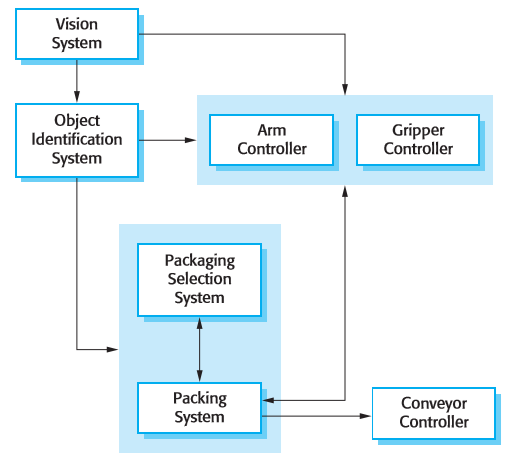
\includegraphics[scale=0.85]{architecture.png}
\caption{Pakkausrobotin arkktehtuurimalli \parencite[s.149]{Sommerville}}
\end{figure}


Kaaviossa esitellään robottisovelluksen jako erilaisiin komponentteihin. Robotti pystyy pakkaamaan kaikenlaisia tavaroita liukuhihnalta. Se käyttää Näkö-komponenttia (\emph{Vision System}) valitakseen erilaisia tavaroita ja tunnistamaan Identifiointi-komponentilla (\emph{Object Identification System}) tavaroiden tyypin. Kun tavara on tunnistettu, se annetaan Pakkaus-komponentille prosessoitavaksi (\emph{Packing Selection System} ja \emph{Packing System}). Tämän jälkeena käsitellään tavara antamalla vastuu käsivarrelle (\emph{Arm Controller}) ja kouralle (\emph{Gripper Controller}), jotka kontrolloivat robotin fysiikka. Lisäksi robotilla tulee olla liukuhihnan hallintakomponentti (\emph{Conveyor Controller}), joka pystyy mahdollisesti pysäyttämään, hidastamaan tai nopeuttamaan linjaston kulkua \parencite[s.148]{Sommerville}.

\section{Web-sovellukset}
WWW:n (World Wide Web) kehityksellä on ollut tärkeä rooli sovelluksien kehityksessä. Alun perin Web oli yliopistojen käytössä datan tallennusta varten ja sillä oli hyvin vähän vaikutusta sovelluksiin. Webin ympärille kirjoitetut sovellukset olivat käynnissä paikallisissa tietokoneissa ja niihin oli pääsy ainoastaan organisaation sisällä. 2000-luvun alussa Web alkoi kehittyä laajemmin. Selaimiin lisätyt ominaisuudet mahdollistivat web-pohjaisten sovellusten käytön siten, että erillisen sovellukselle tarkoitetun käyttöliittymän sijasta voitiin käyttää selainta. Tämä johti monien erilaisten sovelluksien kehitykseen, jotka tarjosivat innovatiivisia palveluita käytettäväksi selaimen kautta. Webin kehityksen myötä selaimet kehittyivät siten, että ne pystyivät ajamaan myös pieniä sovelluksia paikallisesti. Tämä muutti organisaatioiden sekä liiketoiminnan tapoja käyttää sovelluksia. Sen sijaan, että sovellukset olisi asennettu käyttäjien tietokoneille, ne voitiin asentaa suoraan yhdelle web-palvelimelle. Tämä laski myös kustannuksia tehdä muutoksia sovelluksiin. Suurin osa liiketoimien harjoittajista on siirtynyt käyttämään web-pohjaisia sovelluksia \parencite[s.13]{Sommerville}.

Seuraava vaihe web-sovellusten kehityksessä olivat web-palvelut. Web-palvelut ovat sovelluskomponentteja, jotka tarjoavat hyödyllisiä palveluja käytettäväksi muille sovelluksille. Siinä missä web-sovellus tarjoaa käyttöliittymän sovellukselle, web-palvelu tarjoaa rajapinnan käyttöliittymäsovellukselle käytettäväksi. Web-palvelu on yksittäinen osa sovellusta ja sovelluksella voi olla monia web-palveluja käytettävänä. Web-sovelluksien kehitys on mahdollistanut useiden monoliittisten järjestelmien siirtämisen hajautetusti eri palvelimille ympäri maailmaa. Tämä helpottaa sovellusten uudelleenkäytettävyyttä ilman, että koko järjestelmää tarvitsee rakentaa uudelleen \parencite[s.13]{Sommerville}. 


\section{Arkkitehtuurin suunnittelu}

Arkkitehtuurin suunnittelu on luova prosessi, jossa toteutetaan halutun järjestelmän organisointi siten, että se vastaa niin järjestelmän toiminallisiin kuin ei-toiminnallisiin vaatimuksiin. Toiminallisilla vaatimuksilla tarkoitetaan vaatimuksia, jotka määräävät mihin tarkoitukseen järjestelmä tulee ja millaisia ominaisuuksia se tarjoaa. Ei-toiminnallisilla vaatimuksilla tarkoitetaan järjestelmän sisäisiä vaatimuksia, jotka ovat usein näkyvissä vain järjestelmän kehittäjille. Ei-toiminnallisilla vaatimuksilla vastataan siihen, miten järjestelmä tulee rakentaa. Toiminnallisilla vaatimuksilla vastataan siihen, mitä järjestelmän tulisi tehdä. Arkkitehtuurin suunnittelu on usein hyvin paljon sidoksissa siihen, millainen järjestelmä on kyseessä. Sommerville määrittelee arkkitehtuurin suunnittelun olevan enemmänkin sarja erilaisia valintoja kuin, että se olisi ennalta määrättyjen aktiviteettien noudattamista. Sommerville esittelee seuraavat yhdeksän yleistä kysymystä, jotka järjestelmäarkkitehtien on kysyttävä suunnitteluprosessin aikana \parencite[s. 151]{Sommerville}:

\begin{enumerate} 
\item Onko olemassa sovellusarkkitehtuuria, joka voi toimia valmiina pohjana järjestelmälle?
\item Millä tavalla järjestelmä hajautetaan prosessorien tai ytimien kesken?
\item Mitä erilaisia arkkitehtuurimalleja käytetään?
\item Minkä ajatuksen pohjalle järjestelmä rakennetaan?
\item Millä tavalla järjestelmän pääkomponentit hajautetaan alikomponenteiksi?
\item Millaista strategiaa käytetään hallitsemaan komponentteja järjestelmässä?
\item Millainen arkkitehtuurillinen organisointi on paras ei-toiminnallisille vaatimuksille?
\item Millä tavalla arkkitehtuurin suunnittelu evaluoidaan?
\item Miten järjestelmän arkkitehtuuri dokumentoidaan?
\end{enumerate}

Vaikka jokainen järjestelmä on uniikki, on niissä paljon yhteistä arkkitehtuurin suhteen. Esimerkiksi tuotteistetut sovellukset rakennetaan yhden pohja-arkkitehtuurin ympärille, josta toteutetaan erilaisia variaatioita vastaamaan erilaisiin vaatimuksiin. Arkkitehtuuria suunnitellessa tulee päättää, mitä osia arkkitehtuurista voidaan käyttää uudelleen ja mitkä ovat tarkoitettuja vain tietylle asiakasvaatimukselle \parencite[s. 151]{Sommerville}. Järjestelmän arkkitehtuuri voi pohjautua johonkin tiettyyn malliin tai tyyliin. Arkkitehtuurimalli on kuvaus järjestelmän teknisestä organisoinnista. Tällaisia voivat olla esimerkiksi asiakas-palvelin-arkkitehtuuri tai kerrosarkkitehtuuri, johon Sommerville MVC:n luokittelee. Arkkitehtuurin valinnassa tulee ottaa huomioon erityisesti järjestelmän vaatimukset. Sommerville \parencite[s.152]{Sommerville} esittelee viisi pääarvoa, joiden perusteella arkkitehtuurin valintaa voidaan ohjata:

\begin{desclist}
\item[Suorituskyky] Jos suorituskyky on suurimpana vaatimuksena, tulee kriittisimmät operaatiot olla samalla tietokoneella ja arkkitehtuuri jaettu mahdollisimman suuriin komponentteihin, jotta kommunikaatio olisi mahdollisimman suoraviivaista. Useiden pienten komponenttien hajauttaminen usealla tietokoneelle tuo usein ylimääräistä viestintää komponenttien välillä, mikä hidastaa komponenttien yhteisiä operaatioita. 
\item[Tietoturva] Jos tietoturva on suurimpana vaatimuksena, tulee käyttää kerrosarkkitehtuuria, jossa kaikkein kriittisimmät toiminnot on piilotettu alimpiin kerroksiin. Uloimmissa kerroksissa tulee olla tarkat datan validoinnit. 
\item[Turvallisuus] Jos turvallisuuus on suurimpana vaatimuksena, tulee turvallisuuteen liittyvien operaatioiden olla rakennettuna yhden tai mahdollisimman harvan komponentin varaan. Tämän avulla pystytään järjestelmä suojaamaan mahdollisilta järjestelmävirheiltä helposti ja turvallisesti.
\item[Saatavuus] Jos saatavuus on suurimpana vaatimuksena, tulee arkkitehtuuri suunnitella siten, että komponentit tekevät mahdollisimman vähän kriittisiä komponentteja. Tuolloin komponentteja voidaan päivittää ja korvata ilman, että koko järjestelmää tarvitsee pysäyttää. 
\item[Ylläpito] Jos ylläpito on suurimpana vaatimuksena, tulee komponenttien olla mahdollisimman itsenäisiä. Datan tuottajien tulee olla erossa datan käyttäjistä ja jaettuja datamalleja tulee välttää.
\end{desclist}

Yllä esitellyissä arkkitehtuureissa voi kuitenkin olla ristiriitoja. Esimerkiksi suuret komponentit parantavat suorituskykyä ja pienet parantavat järjestelmän saatavuutta. Järjestelmän vaatimukset voivat vaatia kumpaakin, jolloin on tehtävä kompromisseja. Usein kompromissit pystytään saavuttamaan käyttämällä erilaisia arkkitehtuureja järjestelmän eri osissa \parencite[s.152]{Sommerville}. 


\pagebreak

\section{Hajautetut järjestelmät}
Henkilökohtaiselle tietokoneelle käyttöön tarkoitetut järjestelmät sekä sulautetut järjestelmät ovat tyypillisesti rakennettu yhden prosessorin varaan. Niitä ei siis ole hajautettu useiden prosessorien tai ytimien kesken toisin kuin suurempia hajautettuja järjestelmiä. Hajautuksen suunnittelu on yksi avaintekijöitä arkkitehtuurin suunnittelussa, kun järjestelmän koko kasvaa. Käytännössä lähes kaikki suuret tietokonepohjaiset järjestelmät ovat hajautettuja. Ne näyttäytyvät loppukäyttäjälle kuitenkin yhtenä yhtenäisenä järjestelmänä. Hajautetuissa järjestelmissä komponentit voivat olla useilla eri tietokoneilla. Tällöin tulee erityisesti ottaa huomioon niiden välinen kommunikointi, joka hoidetaan verkon yli \parencite[s. 480]{Sommerville}. Coulouris \parencite{Coulouris} esittelee seuraavat hyödyt hajautetuista järjestelmistä:

\begin{desclist}
\item[Resurssien jako] Hajautettu järjestelmä mahdollistaa laitteistojen ja sovellusten resurssien jakamisen. Esimerkiksi tulostimet, tiedostot ja levytila voidaan jakaa tietokoneiden kesken verkon yli.
\item[Avoimuus] Hajautetut järjestelmät ovat usein avoimia ja siten käyttävät standardien mukaisia protokollia. Tällä mahdollistetaan järjestelmän komponenttien yhdistely monien eri tahojen toimesta. 
\item[Rinnakkaisuus] Prosesseja voidaan ajaa rinnakkain verkossa olevien tietokoneiden kesken.
\item[Skaalautuvuus] Hajautetuissa järjestelmissä mahdollistetaan resurssien kasvattaminen lisäämällä tietokoneita vaatimusten muuttuessa. Käytännössä kuitenkin verkko, jolla tietokoneet yhdistetään, saattaa rajoittaa järjestelmän skaalautuvuutta.
\item[Virheiden sieto] Usean tietokoneen käyttö mahdollistaa datan kopioinnin tietokoneiden välillä, jolloin yhden tietokoneen virhetilanteessa voidaan turvautua useampaan muuhun tietokoneeseen. 
\end{desclist}

Suuret hajautetut järjestelmäarkkitehtuurit ovat yllä mainittujen hyötyjen takia korvanneet suurimman osan vanhemmista järjestelmistä, jotka kehitettiin 1990-luvulla. On kuitenkin vielä paljon henkilökohtaisia sovelluksia, jotka toimivat yhdellä koneella. Tällaisia ovat esimerkiksi erilaiset kuvankäsittelyohjelmat. Suurin osa sulautetuista järjestelmistä on myös yhden prosessorin varaan rakennettuja \parencite[s. 480]{Sommerville}. 

Hajautetut järjestelmät ovat yleensä monimutkaisempia kuin yhden prosessorin ympärille rakennetut järjestelmät. Tämä tekee niistä vaikeampia suunnitella, toteuttaa ja testata. Erityisen vaikeaa on ymmärtää järjestelmän yhtenäisiä toimintoja, jotka eivät riipu yksittäisistä komponenteista vaan monien komponenttien tarjoamasta yhtenäisestä toiminnosta. Tämä johtuu kommunikaatiosta niin järjestelmän yksittäisen komponenttien välillä kuin järjestelmän infrastruktuurista. Esimerkiksi yksittäisen prosessorin ympärille rakennetun järjestelmän suoristuskyvyn perustana on prosessorin nopeus, mutta hajautetun järjestelmän kohdalla tulee ottaa huomioon verkon kuorma, verkon nopeus sekä kaikkien tietokoneiden nopeus, jotka ovat osa järjestelmää. WWW on rakennettu hajautettujen järjestelmien ympärille ja on hyvä esimerkki siitä, kuinka epävakaa ja ennalta arvaamaton se luonteeltaan on. Vastausajat riippuvat arkkitehtuurista, verkon kuormasta sekä yksittäisten palvelimien kuormasta \parencite[s. 481]{Sommerville}.  

\section{Hajautetut järjestelmät ja Internet}

Internetin päälle rakennetut hajautetut järjestelmät käyttävät asiakas-palvelin-arkkitehtuuria. Asiakas/palvelin järjestelmissä käyttäjä kommunikoi paikallisesti omalle koneelleen asennetun sovelluksen avulla. Tällaisia ovat esimerkiksi selaimet ja erilaiset sovellukset älypuhelimessa. Kommunikoinnissa käyttäjän sovellus ottaa yhteyden verkon yli toiseen sovellukseen, joka on käynnissä toisella tietokoneella (palvelin). Palvelin tarjoaa erilaisia palveluita, kuten esimerkiksi web-sivuja. Asiakas/palvelin -arkkitehtuuri on hyvin geneerinen ja yleisesti käytössä oleva arkkitehtuuri. Se ei rajoitu sovelluksiin, jotka on hajautettu useille tietokoneille, vaan sitä voidaan käyttää myös arkkitehtuurina jakamaan sovellukset loogisesti yhdellä tietokoneella \parencite[s.488]{Sommerville}.

Järjestelmät, jotka käyttävät asiakas-palvelin-arkkitehtuuria, koostuvat useista palveluista. Palvelut on usein jaettu myös usealle tietokoneelle. Sommerville jakaa asiakas-palvelin-arkkitehtuurin mallin kolmeen osaan \parencite[s. 161]{Sommerville}: 

\begin{enumerate} 
\item Useita palvelimia, jotka tarjoavat palveluita muille komponenteille. Tällaisia ovat esimeriksi tulostinpalvelut tai tiedostojenhallintaan erikoistuneet tiedostopalvelut.
\item Useita asiakasjärjestelmiä, jotka kutsuvat palvelimien tarjoamia palveluita. Normaalisti on useita asiakasjärjestelmän ilmentymiä, jotka käyttävät rinnakkain palvelimia.
\item Verkko, jonka kautta datan siirto palvelimien ja asiakasjärjestelmien välillä hoidetaan. Suurin osa asiakas/palvelin -järjestelmistä on hajautettu ja ne luovat yhteydet käyttäen apunaan useita protokollia.
\end{enumerate}

Tärkeimpänä etuna asiakas-palvelin-arkkitehtuurissa on komponenttien itsenäisyys sekä hajautus. Palveluja ja palvelimia voidaan vaihtaa tai muokata ilman, että vaikutetaan muihin järjestelmän osiin. Palvelimen ei myöskään tarvitse tietää asiakassovelluksen identiteetistä mitään. Asiakassovellukselle riittää yleensä vain palvelimien ja niissä ajettavien palvelujen nimet. Asiakas kutsuu palvelimen tarjoamaa palvelua käskemällä tätä suorittamaan halutun ohjelmakoodin käyttäen apunaan esimerkiksi HTTP-protokollan GET-viestiä, jota käytetään WWW:ssä pyytämään dataa palvelimelta. Pääasiallisesti asiakas lähettää pyynnön palvelimelle ja odottaa kunnes palvelin vastaa viestiin.

\begin{figure}[h]
\centering
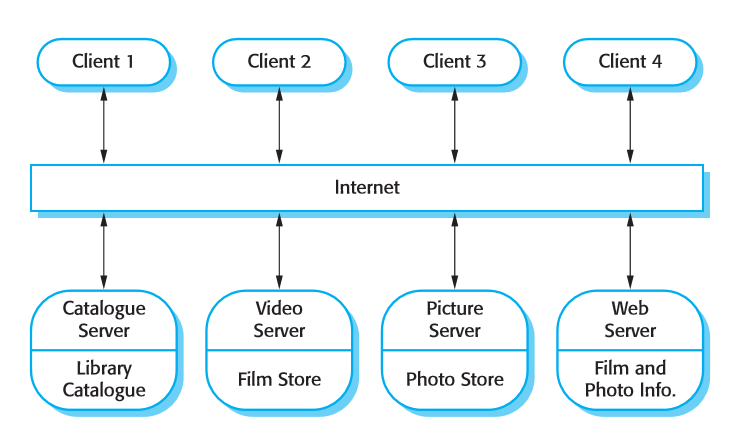
\includegraphics[scale=0.85]{clientserver.png}
\caption{Sommervillen esimerkki elokuvakirjaston asiakas-palvelin-arkkitehtuurista \parencite[s.162]{Sommerville}}
\end{figure}

Yllä esitetyssä mallissa esitellään monen käyttäjän web-pohjainen järjestelmä elokuvien ja kuvien tarjontaan. Järjestelmässä useat palvelimet hallitsevat ja tarjoavat erityyppisiä multimediatiedostoja. Videotiedostojen tarjonta tulee olla erittäin nopeaa ja synkronista. Jotta tähän pystytään, tulee videotiedosto pakata pienemmäksi ja tarjota pienemmällä resoluutiolla. Lisäksi videoiden formaatit voivat vaihdella, jolloin videoille tarkoitetun palvelimen tulee pystyä tarjoamaan palvelua, jossa erilaisia videoformaatteja voidaan pakata ja purkaa. Kuvia on kuitenkin sopivaa tarjota suurilla resoluutioilla, joten niiden käsittely voidaan hoitaa erillisellä palvelimella. Näin ei tarvitse kuormittaa yhtä palvelinta kahdella toisistaan poikkeavalla prosessilla. Katalogin tulee pystyä käsittelemään useita erilaisia kyselyjä sekä tarjota yhteyksiä järjestelmiin, jotka hallitsevat esimerkiksi elokuvien tietoja sekä valokuvien myyntiä. Asiakassovellus on yksinkertainen käyttöliittymä, joka on rakennettu web-selaimeen ottamaan yhteyksiä palveluihin \parencite[s. 163]{Sommerville}. 

\chapter{Internet}
Internet ja sen arkkitehtuuri on syntynyt hyvin pienistä saavutuksista. Internetin taustalla ei ole alun perin ollut minkäänlaista suurempaa suunnitelmaa. Tutkiessamme Internetin arkkitehtuuria tulee muistaa, että tekniset muutokset ovat jatkuvia tietotekniikan alalla. Monet arkkitehtuurilliset ratkaisut, jotka olivat suosiossa muutamia vuosia sitten, ovat nyt jo vanhentuneet. Toisaalta ratkaisut, jotka tänä päivänä nähdään hyvinä, voivat jo huomenna olla huonoja. Voidaan sanoa, että ainut asia joka Internetin suhteen pysyy on jatkuva muutos. Internet-yhteisön  monet jäsenet väittävät, että Internetillä ei ole arkkitehtuuria, mutta kuitenkin eräänlaisia perinteitä, johon koko Internet pohjautuu \parencite{constant_change}. Väite voidaan kuitenkin kumota, sillä Internet perustuu asiakas-palvelin-arkkitehtuuriin \parencite[s. 162]{Sommerville}.
Internetin tavoite on tarjota yhteydet, jossa käytetään pohjana Internet Protokollaa (IP). Monien Internet-yhteisön jäsenien mielestä tärkeää ei ole se millä tavalla yhteydet luodaan verkon sisällä, vaan se millä tavalla yhteyksien alku- ja loppupää käyttäytyvät. Tähän tärkeimpänä argumenttina pidetään sitä, että useat tarvittavat toiminnallisuudet voidaan toteuttaa vain IP:tä käyttävien systeemien puolella. Jokainen hyvin suunniteltu verkko sisältää mahdollisuuden jollakin tasolla epäonnistua viestin kuljettamisessa. Tällaisen ongelman kanssa tulisi toimia siten, että vastuu kommunikaation eheydestä annetaan ulkopuolisille sovelluksille. Nykyinen Internetin eksponentaalinen kasvu näyttää kuitenkin sen, että yhteydet ovat paljon arvokkaampia kuin yksittäiset sovellukset. Tällaiset yhteydet vaativat yhteistyötä palveluntarjoajien ja televiestintäympäristöjen välille \parencite{constant_change}. 

Yleisesti on haluttua, että olisi vain yksi protokolla, jonka kautta yhteydet voidaan muodostaa. Tämän protokollan päälle voidaan kuitenkin rakentaa monia muita protokollia, jotka hoitavat muita erilaisia tarpeita. Käytännössä on ainakin kaksi syytä, miksi verkkoprotokollien tasoja tarvitaan useita. Esimerkiksi eri IP:stä voidaan haluta vaihtaa toiseen versioon. Myös uudet vaatimukset voivat synnyttää uusia protokollia. Internetin protokollien tulee olla täysin riippumattomia laitteistosta. Tällöin Internet voidaan toteuttaa minkä tahansa digitaalisen teknologian päälle \parencite{constant_change}.

\section{Historia}
Internetin historia on lähtöisin tarpeesta luoda yhteyksiä tietokoneiden välille, joiden avulla voidaan luoda verkkoja. Verkkojen kautta erilaiset sovellukset voivat keskustella keskenään. Tämä on johtanut tarpeeseen luoda standardit, jotka määrittävät sen millä tavalla yhteyksiä tulisi luoda ja ylläpitää. TCP (Transmission Control Protocol) on standardi, joka määrittää yhteyden luonnin tietokoneiden välillä sekä niiden välisen kommunikoinnin. TCP:n avulla sovellukset pystyvät lähettämään dataa toisilleen verkon yli. TCP kehitettiin Yhdysvaltain asevoimien tutkimusorganisaatiossa DARPA:ssa (Defense Advanced Research Projects Agency) \parencite{tcp1_1}. 

\section{TCP}
TCP on tarkoitettu toimivan eri tasoihin jaetussa protokollien hierarkiassa, joka tukee verkkosovelluksia. Sen tarkoitus on pystyä toimimaan monien alemman tason protokollien päällä ottamatta kantaa siihen, käytetäänkö yhteyden muodostuksessa esimerkiksi paketti- tai piirikytkentää. DARPA määrittää eri protokollien tasot seuraavasti:


\begin{figure}[h]
\centering
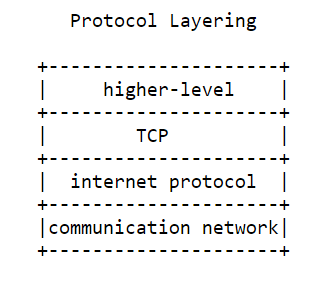
\includegraphics[scale=0.85]{protocol_layering.PNG}
\caption{\parencite{tcp1_1}}
\end{figure}


TCP on rakennettu Internet Protokollan päälle, joka tarjoaa TCP:lle työkalut määrittää lähettäjän ja vastaanottajan osoitteet erilaisissa verkoissa. Internet Protokolla hoitaa myös mahdollisten TCP-segmenttejen pirstaloinnin ja uudelleenkokoamisen, jolloin TCP:n ei tarvitse näistä huolehtia. Se myös pitää mukanaan tiedon TCP-segmenttejen järjestyksestä, tietoturvamäärityksistä sekä lajittelusta. TCP tarjoaa rajapinnan luotettavalle yhteydelle useista verkoista koostuvassa ympäristössä \parencite{tcp1_1} 

TCP koostuu kahdesta rajapinnasta, joista toinen toimii käyttäjälle tai sovellukselle ja toinen alemman tason protokollille kuten Internet Protokollalle. Sovelluksille tarkoitettu rajapinta koostuu vastaavista kutsuista, joita käyttöjärjestelmä tarjoaa tiedostojen hallintaan. Esimerkiksi se sisältää kutsut yhteyden avaamiseen ja sulkemiseen sekä datan vastaanottoon ja lähetykseen yhteyden läpi. TCP pystyy myös asynkronisesti kommunikoimaan sovelluksien kanssa. Rajapinta alemmille protokollille on yleisesti määrittelemätön, mutta se olettaa rajapinnassa olevan mekanismin, jossa kaksi tasoa pystyvät asynkronisesti siirtämään dataa toistensa välillä. Yleensä kyseinen määrittely oletetaan löytyvän alemman tason protokollalta. TCP on tarkoitettu toimivan geneerisessä ympäristössä, mutta yleisesti voidaan olettaa alemman tason protokollan olevan Internet Protokolla \parencite{tcp1_4}.

TCP:n tärkein tehtävä on tarjota turvallinen ja luotettava yhteys kahden prosessin välille. Tarjotakseen tällaisen palvelun, tulee tietyt osa-alueet toteutua. IETF \parencite{tcp1_4} määrittää TCP:n toteuttamat osa-alueet seuraavasti:

\begin{desclist}
\item[Datan siirto] TCP pystyy lähettämään jatkuvasti paketteja kummankin käyttäjän suuntaan. Joskus käyttäjien tulee varmistaa, että kaikki lähetetty data on lähetetty vastaanottajalle. Tähän tarkoitukseen on kehitelty \emph{push} -toiminto, joka käskee TCP:tä
lähettämään datan vastaanottajalle.
\item[Luotettavuus] TCP:n tulee pystyä selviytymään tilanteesta, jossa data on jollain tavalla korruptoitunut tai hävinnyt. Tämä on ratkaistu lisäämällä jokaiseen pakettiin sekvenssinumero ja jokaisessa viestissä vaaditaan kuittausta vastaanottajalta. Jos kuittausta ei jostain syystä saada, lähetetään paketti uudelleen. Vastaanottajan puolella sekvenssinumeron avulla pystytään päättelemään oikea järjestys.
\item[Datavirran hallinta] TCP antaa vastaanottajalle mahdollisuuden rajata datamääriä. Tämä mahdollistetaan antamalla vastaanottajalle mahdollisuus lähettää kuittausviestin mukana ikkuna, joka määrittää rajat datalle.
\item[Kanavointi] Koska yhden isäntäkoneen on mahdollista palvella useita TCP-yhteyksiä rinnakkain, tulee TCP:n tarjota lista osoitteita ja portteja yksittäistä palvelinta kohden. Jokaiselle yhteydelle luodaan soketti (socket). Sokettipari muodostaa uniikin yhteyden, missä yksittäistä sokettia voidaan myös käyttää moniin eri yhteyksiin rinnakkain. Hyvänä esimerkkinä yhden soketin jakamisesta ovat erilaiset prosessit sovelluksen logeja varten. Erillisiin portteihin liittäminen hoidetaan aina jokaisen isäntäkoneen toimesta.
\item[Yhteydet] Luotettavuuden ja kanavoinnin toteutus vaatii TCP:ltä erillisen tilan alustamista ja ylläpitoa jokaiselle datavirralle. Tietoa soketeista, sekvenssinumeroista ja ikkunoiden koosta kutsutaan yhteydeksi. Jokainen yhteys määritellään sokettiparin perusteella. Kun kaksi prosessia haluaa kommunikoida keskenään, kummankin TCP:n tulee ensin luoda yhteys, jolloin kummankin tila alustetaan. Kun yhteys on valmis, se terminoidaan tai suljetaan resurssien vapauttamiseksi. Koska yhteydet luodaan epävakaan internet-yhteyden sekä epäluotettavien prosessien välille, TCP käyttää kättelymekanismia yhteyden muodostamisessa. Tämän avulla vältetään virheelliset yhteydenmuodostukset.
\item[Priorisointi ja tietoturva] TCP:n käyttäjät voivat hallita priorisointia sekä tietoturvaa erilaisilla arvoilla. Tällainen on esimerkiksi TCP-oktetin sisältämät ensimmäiset kolme bittiä, jotka määrittävät oktetin tärkeysjärjestyksen.
\end{desclist}


TCP:n oletetaan olevan tavallinen moduuli käyttöjärjestelmässä. Käyttäjien tulee pystyä hallitsemaan TCP:tä niin kuin mitä tahansa tiedostojärjestelmää. Se pystyy myös kutsumaan muita käyttöjärjestelmän toimintoja. Rajapinta itse verkkoon tulee kuitenkin toteuttaa laitteen ajurissa. TCP ei kuitenkaan kutsu ajurin rajapintaa suoraan, vaan käyttää Internet Protokollaa. Internet Protokolla sen sijaan kutsuu mahdollisen alemman tason ajurin rajapintaa. Käyttäjälle tarkoitettu rajapinta toteutetaan TCP:ssä siten, että sen kutsut ovat vastaavia kuin muissakin käyttöjärjestelmän ohjelmien tarjoamissa kutsuissa. TCP:n käyttäjille tarjoamassa rajapinnassa kutsut ovat seuraavat \parencite{tcp2_3}:

\begin{desclist}
\item[OPEN] Avaa yhteyden
\item[CLOSE] Sulkee yhteyden
\item[SEND] Lähettää dataa
\item[RECEIVE] Ottaa vastaan dataa
\item[STATUS] Palauttaa yhteyden tilan
\end{desclist}

Kutsut ovat täysin verrattavissa käyttöjärjestelmän käyttäjäsovelluksien kutsuihin. Tällaisia ovat esimeriksi tiedostojen luku- ja kirjoituskutsut. Rajapinnan tarkoituksena on tarjota kutsuja datagrammejen lähetykseen ja vastaanottamiseen kaikkien osapuolien välillä, jotka on kytketty Internettiin. Kutsujen avulla voidaan viedä parametreissa erilaista tietoa kuten osoite, palvelun tyyppi, järjestysnumero ja muita datagrammejen hallintaan liittyviä tietoja. Datagrammi on yksikkö, joka mahdollistaa datan siirtämisen itsenäisesti kahden tietokoneen välillä ilman, että se on riippuvainen aiemmista tapahtumista \parencite[s.33]{datagram}.

\section{Internet Protokolla}

Internet Protokolla on tarkoitettu käytettäväksi tietokoneiden välisiin verkkoihin, joissa on käytössä pakettikytkentä. Se tarjoaa toteutuksen siirtämään datagrammeja käyttäjien välillä. Se toteuttaa myös pitkien datagrammejen pirstaloinnin pienempiin osiin tarvittaessa, jos dataa halutaan siirtää verkkojen läpi, jossa vain pienet paketit ovat sallittuja. Internet Protokolla ei ota kantaa datan luotettavuuteen, datavirran hallintaan tai järjestykseen. Tämä jätetään ylemmän tason protokollien hoidettavaksi. Esimerkiksi TCP-moduuli kutsuu Internet moduulia ottamaan haltuun TCP-segmentin, joka sisältää otsikon ja lähettäjän datan. Otsikko sisältää osoitteen ja muut tarvittavat parametrit. Tämän jälkeen Internet-moduuli luo datagrammin ja kutsuu paikallista verkkorajapintaa lähettämään datagrammin eteenpäin \parencite{internet_protocol}.

Internet Protokolla toteuttaa kaksi toiminnallisuutta: osituksen ja osoitteistuksen. Datagrammin otsikoissa tulleiden tietojen perusteella osataan lähettää data oikeaan paikkaan sekä pirstaloida data sopivaksi verkolle. Internet Protokolla käsittelee jokaista datagrammia erillään ilman riippuvuuksia muista datagrammeista. Internet Protokolla käyttää neljää palvelua: Palvelutyyppi, Elinkaari, Vaihtoehdot ja Tarkistussumma. Palvelutyyppi on abstrakti tai geneerinen lista parametrejä, jotka määrittää verkolle minkä tyyppinen palvelu on kyseessä. Yhdyskäytävät käyttävät tätä informaatiota valitsemaan oikeat parametrit tietylle verkolle tai määrittämään seuraavan verkon mihin hypätä. Yhdyskäytävillä tarkoitetaan verkon solmua, joka mahdollistaa siirtymisen toiseen verkkoon. Solmut voivat olla esimerkiksi tietokoneita. Elinkaarella tarkoitetaan ylärajaa, jonka aikana datagrammin tulee saavuttaa määränpäänsä. Jos määränpäätä ei saavuteta, datagrammi tuhotaan. Yläraja määritetään lähettäjän toimesta ja sitä vähennetään siirron aikana. Datagrammi tuhoutuu saavuttaessaan arvon nolla \parencite{internet_protocol}. Vaihtoehdot ovat käytössä erityisissä tilanteissa. Tällaisia ovat esimerkiksi tietyt ohjaukset verkossa tai lisäykset tietoturvaan. Tarkistussummalla varmistetaan, että datagrammi on siirretty onnistuneesti. Datagrammin sisältö voi kuitenkin sisältää virheitä. Jos Tarkistussummassa on virheitä, datagrammi tuhotaan välittömästi. 

Internet Protokolla ei tarjoa luotettavaa kommunikaatioyhteyttä. Se ei sisällä alku- ja loppupään kuittauksia eikä se ota kantaa datan eheyteen. Se ei myöskään sisällä uudelleenlähetyksiä tai muuta datavirran hallintaa \parencite{internet_protocol}.


\section{HTTP-protokolla}
HTTP (Hypertext Transfer Protocol) on ollut Internetin WWW:n käytössä vuodesta 1990 lähtien. HTTP:n yhtenä tarkoituksena on siirtää hypertekstidokumentteja järjestelmien välillä. Hypertekstillä tarkoitetaan tietokoneissa käytettyä tekstiä, jossa mahdollistetaan ristiviittauksia dokumenttien välillä. Näitä viittauksia kutsutaan hyperlinkeiksi \parencite{hypertext}. HTTP on sovellustason protokolla ja se käyttää alemman kuljetuskerroksen protokollia yhteyden luomisessa. WWW:ssä HTTP käyttää kuljetuskerroksen TCP-protokollaa \parencite{w3http}. HTTP on geneerinen sekä tilaton ja sitä voidaan käyttää muuhunkin kuin hypertekstin siirtämiseen ylätunnisteiden, pyyntöjen sekä virhekoodien kautta. Tällaisia ovat esimerkiksi nimipalvelimet ja jaetut oliopohjaiset hallintajärjestelmät. HTTP-protokolla mahdollistaa järjestelmien rakentamisen riippumattomana siirrettävästä datasta \parencite{http}. HTTP tuo sovelluksille mahdollisuuden kommunikoida avoimella joukolla menetelmiä ja ylätunnisteita, jotka määrittävät itse HTTP-viestin tarkoituksen. HTTP käyttää URI:n spesifikaatiota määrittämään resurssien sijainnin \parencite{uri}.

\begin{figure}[h]
\centering
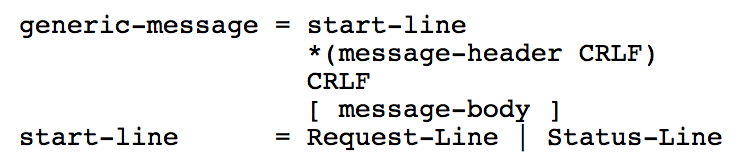
\includegraphics[scale=0.85]{generic_message.png}
\caption{HTTP-viesti kokonaisuudessaan \parencite{httprequest}}
\end{figure}

HTTP-viestit koostuvat asiakaspuolen viesteistä sekä palvelimen vastauksista asiakkaalle. Molemmat viestit sisältävät aloitusrivin, tyhjän tai useamman ylätunnisteen, tyhjän rivin (CRLF) ja mahdollisen lähetettävän viestin. CRLF määrittää rivinvaihdon ja palvelimen on pystyttävä protokollan datavirtaa luettaessa huomioimaan se. Esimerkiksi datavirtaa luettaessa, jos viesti alkaa CRLF:llä, se tulee hylätä. HTTP-viesti sisältää erilaisia ylätunnisteita (header), joiden avulla voidaan viedä ylimääräistä tietoa HTTP-pyynnöstä sekä asiakaspäästä. Ylätunnisteita voi olla useita yhdessä HTTP-viestissä. Viestikentässä (\emph{message-body}) viedään tietyn viestin sisältö, jos sellainen on viestissä mukana \parencite{httprequest}. Viestikentän olemassaolo määritetään pituuskentässä (\emph{Content-Length}) tai kentässä, joka määrittää siirron enkoodauksen (\emph{Transfer-Encoding}). HTTP-pyynnön ei tule sisältää viestikenttää, jos esimerkiksi enkoodauksen kenttä löytyy pyynnöstä ja se sisältää minkä tahansa muun arvon kuin "identity". Seuraavaksi esitellään yleisellä tasolla esimerkki millä tavalla asiakas saa HTTP-palvelimelta vastauksena hypertekstidokumentin.

Yhteyden luonnissa asiakas luo TCP/IP-yhteyden palvelimen ja asiakkaan välille käyttäen osoitteessa määriteltyä porttinumeroa. Jos porttinumeroa ei ole annettu, HTTP olettaa porttinumeron olevan 80. Asiakas lähettää pyynnön, joka koostuu yhdestä rivistä ASCII-merkkejä. Pyyntö sisältää sanan "GET", välilyönnin sekä dokumentin osoitteen. Dokumentin osoitteen tulee olla yksi yhtenäinen sana. Kaikki ylimääräiset sanat, jotka löydetään dokumentin osoitteesta, jätetään huomioimatta tai ne tulkitaan HTTP-spesifikaation mukaisesti \parencite{w3http2}. Vastaus yksinkertaiseen GET-viestiin voi sisältää esimerkiksi HTML-pohjaisen (Hypertext Markup Language) ASCII datavirran. HTML-kieltä käytetään julkaisemaan hypertekstidokumentteja WWW:ssä. HTML:n pohjana on käytetty SGML:ää, joka on standardi määrittelemään merkkauskieliä \parencite{sgml}. HTML-dokumentit ovat siis SGML-dokumentteja, jotka toteuttavat SGML:n määritelmät. Hyvin toteutetut asiakassovellukset lukevat koko dokumentin mahdollisimman nopeasti, jolloin käyttäjän laukaisemat toiminnot, toteutetaan vasta dokumentin prosessoinnin jälkeen. TCP/IP yhteys suljetaan palvelimen toimesta kun koko dokumentti on siirretty \parencite{w3http}

HTTP-protokollan alkuperäinen toteutus on tarkoitettu yksisuuntaiseksi, jolloin asiakkaan tulee lähettää aina pyyntö palvelimelle vastaanottaakseen dokumentteja. Palvelimen ei ole tarkoitus syöttää tietoa suoraan asiakkaalle ilman tämän pyyntöä. Tästä syystä asiakkaan on aina toistuvasti pyydettävä tietoja erikseen. Tätä kutsutaan ”pollaukseksi” (polling). Tämä kuitenkin luo paljon kuormaa ja ylimääräisiä kyselyitä palvelimelle niissä tilanteissa, jossa pyynnölle tarkoitettu vastaus ei ole vielä valmis. Tämän ratkaisemiseksi HTTP-protokollaan on toteutettu mahdollisuus lähettää viestejä palvelimelta asiakkaalle. Tämä mahdollistaa kaksisuuntaista viestintää asiakkaan ja palvelimen välillä, jolloin asiakkaan ei tarvitse pollata jokaista muutosta. Tyypillisimmät toteutukset ovat pitkä pollaus  (\emph{HTTP Long Polling}) ja HTTP-virta (\emph{HTTP-Streaming}) . Pitkässä pollauksessa palvelin pyrkii pitämään yhteyden auki selaimelle ja vastaamalla vasta, kun pyyntö on prosessoitu. Tämän jälkeen yhteys suljetaan. HTTP-virrassa palvelin pitää pyynnön auki niin kauan kuin vain mahdollista eikä koskaan terminoi pyyntöä tai sulje yhteyttä. HTTP-virrassa vastauksia lähetetään osissa \parencite[s. 2]{long_polling}. Edellä mainittuja toteutuksia ei kuitenkaan ole tarkoitettu alkuperäiseen HTTP-toteutukseen. HTTP on alun perin tarkoitettu yksisuuntaiseen kommunikaatioon, mistä syystä kaksisuuntaisen kommunikaation lisääminen HTTP:hen tuottaa ongelmia. Alla esitellään kummankin toteutuksen ongelmat.


\textbf{Pitkä pollaus}:
\begin{desclist}
\item[Otsikoiden kuormitus] Jokainen pyyntö on kokonainen HTTP-viesti ja sisältää kaiken datan otsikoita myöten. Tästä syystä lyhyissäkin viesteissä siirrettävät datamäärät ovat isoja, jotka johtavat verkon kuormitukseen.
\item[Maksimaalinen viive] Kun pyyntö on lähetetty asiakkaalle, tulee palvelimen odottaa seuraava pyyntöä ennen kuin voidaan lähettää seuraavaa viesti. Tämä johtaa lukuisiin ajallisesti pidempiin viesteihin.
\item[Yhteyksien luonti] Yhteyksiä joudutaan sulkemaan ja availemaan useasti
\item[Resurssien jakaminen] Käyttöjärjestelmät sekä sovellukset pyrkivät pitämään TCP-yhteyksien resurssit minimaalisina. Tästä syystä vastaan tulee erilaisia rajoituksia palvelimien yhteyksien hallinnassa.
\item[Yhteyksien heikentäminen] Suuressa kuormassa toimiva asiakas ja palvelin pyrkivät alentamaan tehokkuutta viestin hitauden kustannuksella.
\item[Aikakatkaisut] Jokaiselle pyynnölle muodostetaan aikaraja, jolloin yhteys katkaistaan. Tämä raja asetetaan usein hyvin korkealle. Useissa selaimissa on kuitenkin asetettu normaaliksi rajaksi 300 sekunttia ja verkkojen infrarstruktuurissa aikaraja on usein paljon pienempi. Tästä syystä yhteyksiä joudutaan väistämättä katkaisemaan pitkien pyyntöjen aikana.
\item[Asiakaspuolen rajoitteet] Asiakkaalla ei ole tapaa ilmoittaa pitkästä pollauksesta, vaan se toteutetaan aina palvelimen toimesta. Asiakaspuolen tulee siis olettaa pyyntöjen kestävän odotettua kauemmin. Tämä voi olla usein ongelmallista erilaisissa toteutuksissa.
\end{desclist}

\textbf{HTTP-virta}:
\begin{desclist}
\item[Välipalvelimet] HTTP-protokolla mahdollistaa välipalvelimien kuulumisen mukaan datan lähetykseen asiakkaan ja palvelimen välissä. Välipalvelimilla ei ole vaatimusta suoraan siirtää vastausta asiakkaalle. Välipalvelimien sallitaan myös puskuroida vastaukset ennen kuin ne lähetetään edelleen eteenpäin. HTTP-virta ei toimi tällaisessa tilanteessa.
\item[Maksimaalinen viive] Täydellisessä verkossa HTTP-virran keskimääräinen ja maksimaalinen viive on yksi siirto verkossa. Todellisuudessa maksimaalinen viive on kuitenkin suurempi johtuen verkon ja selaimien rajoituksista. Selaimien tekniikat, jotka terminoivat HTTP-virran yhteyksiä, ovat usein kytköksissä JavaScript tai DOM (Document Object Model) elementteihin, jotka kasvattavat kokoaan jokaisesta uudesta viestistä. Välttääkseen hallitsemattoman muistin käytön selaimessa, tulee HTTP-virran katkaista yhteys välillä ja lähettää uusi pyyntö uuden virran alustamiseksi.
\item[Asiakkaan puskurointi] HTTP:ssa ei ole vaatimusta asiakaspäälle luoda dataa osittaisista HTTP-vastauksista. Jos esimerkiksi vastaus lähetetään paloissa, jotka sisältävät yksittäisen osan javascriptiä, ei selaimelta vaadita osan ajoa ennen kuin koko vastaus on saatu.
\item[Datan paloittelu] Vastauksien muuttaminen sovellukselle ajettavaksi tulee tehdä sovellustasolla. HTTP-protokollan viestejä ei voida suoraan tulkita sovellusviesteiksi, koska välipalvelimet saattavat muuttaa virran viestien rakennetta. Tämä ongelma ei ole läsnä pitkässä pollauksessa, koska siinä jokainen viesti on oma kokonainen HTTP-pyyntö \parencite[s. 2]{long_polling}. 
\end{desclist}

Yllä esitetyistä ongelmista johtuen kaksisuuntaista kommunikaatiota HTTP:n päällä ei voi tutkielman kannalta luotettavasti käyttää kaksisuuntaisen kommunikaation toteuttamiseen sen epävarmuuden vuoksi.

!
\section{Web-soketti protokolla}
Koska HTTP:ta ei oltu alun perin tarkoitettu kaksisuuntaiseen kommunikaation, tehtiin useat aiemmat teknologiset ratkaisut tehokkuuden ja toimintavarmuuden väliltä. Tämän pohjalta on kehitetty web-soketti protokolla. Web-soketti protokolla on itsenäinen TCP-pohjainen protokolla. Sen avulla mahdollistetaan kaksisuuntainen kommunikaatio palvelimen ja asiakkaan välillä. Protokollaa voidaan käyttää niin tavallisissa web-sivustoissa kuin peleissäkin. Se on suunniteltu erityisesti syrjäyttämään olemassa olevia kommunikointiteknologioita, jotka käyttävät HTTP:ta datan siirrossa. Se on myös luotu toimimaan ympäristöissä, joissa käytetään HTTP:tä. Web-soketteja käytetään oletetusti HTTP-porttejen 443 ja 80 yli. HTTP ei kuitenkaan rajoita web-sokettejen toteutusta. Web-soketti käyttää yksittäistä TCP-yhteyttä lähettäen dataa kumpaankin suuntaan. Protokollassa on kaksi osaa: kättely ja datan siirto \parencite[s. 1.1]{websocket}.

Kättely ei ole riippuvainen HTTP-protokollasta, mutta se on rakennettu toimimaan HTTP-pohjaisten protokollien kanssa. Tässä tutkielmassa keskitytään kättelyyn HTTP-protokollan näkökulmasta. Alla olevassa esimerkissä selain aloittaa kättelyn kutsumalla HTTP-protokollan mukaisesti GET-kutsua. Tämän jälkeen selain vastaa kättelyviestillä, jossa protokolla vaihdetaan käyttämään web-sokettia \parencite[s. 1.1]{websocket}:

\begin{lstlisting}[language=Smalltalk]
        GET /chat HTTP/1.1
        Host: server.example.com
        Upgrade: websocket
        Connection: Upgrade
        Sec-WebSocket-Key: dGhlIHNhbXBsZSBub25jZQ==
        Origin: http://example.com
        Sec-WebSocket-Protocol: chat, superchat
        Sec-WebSocket-Version: 13
\end{lstlisting}

Palvelimelta tuleva vastaus kättelyyn näyttää seuraavalta:
\begin{lstlisting}[language=Smalltalk]
         HTTP/1.1 101 Switching Protocols
        Upgrade: websocket
        Connection: Upgrade
        Sec-WebSocket-Accept: s3pPLMBiTxaQ9kYGzzhZRbK+xOo=
        Sec-WebSocket-Protocol: chat
\end{lstlisting}

Kun asiakas ja palvelin ovat kummatkin lähettäneet kättelyviestinsä ja kättely on onnistunut, alkaa datan siirto. Tuolloin asiakkaan ja palvelimen välillä on yhteys, jonka avulla kummatkin osapuolet voivat lähettää toisilleen viestejä suunnasta riippumatta \parencite[s. 1.2]{websocket}. 


\chapter{MVC}
MVC-arkkitehtuurin perusajatus on erottaa käyttöliittymä sovelluslogiikasta ja
näin tehdä sovelluksesta helposti ylläpidettävä kolmen eri komponentin avulla:
Malli (Model), Näkymä (View) ja Ohjain (Controller). Jokainen komponentti on
erikoistunut sovelluksessa johonkin tiettyyn tehtävään. Mallin tehtävänä on
hallita sovelluksen tilaa ja vastata sen käsittelemästä datasta Ohjaimelle ja Näkymälle.
Näkymän tehtävänä on taas näyttää sovelluksen käyttöliittymä ja sitä kautta Mallin dataa. 
Ohjaimen tarkoitus on ottaa vastaan syötteitä käyttäjältä käskien Mallia ja Näkymää muuttumaan tarvittaessa.


\begin{figure}[h]
\centering
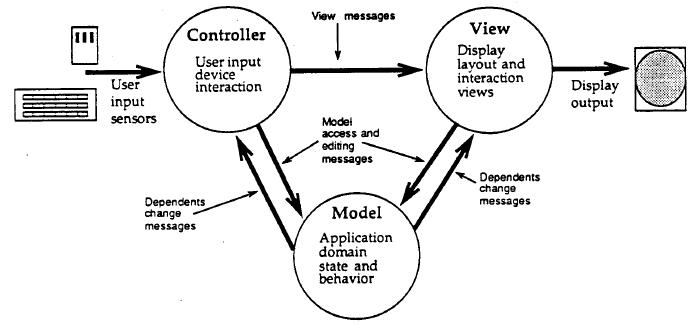
\includegraphics[scale=0.85]{krasner_mvc.jpg}
\caption{Model-View-Controller State and Message Sending \parencite[s. 5]{krasner_desc}}
\end{figure} 
Jokaisella komponentilla on oma rajattu tehtävänsä ja ohjelmakoodi tulee jakaa näiden komponenttien kesken. Jotta MVC:tä pystyttäisiin käyttämään
tehokkaasti, tulee ymmärtää komponenttien työnjako sekä se kuinka komponentit kommunikoivat keskenään \parencite{burbeck}. 

Luodessamme MVC-arkkitehtuurin toteuttavia komponentteja, tulee ne periä jostakin abstraktista pohjaluokasta (Model, View tai Controller), joka määrittelee kyseisen komponentin käyttäytymisen MVC:ssä \parencite[s. 5]{krasner_desc}. Tässä kappaleessa käydään jokaisen komponentin toteutus erikseen läpi käyttäen Smalltalk-ohjelmointikieltä. Lähteenä käytetään Krasnerin julkaisua \parencite{krasner_desc}.

Yleisesti MVC-komponenttien toimintaa kuvaavassa esimerkissä käyttäjältä tulee jokin syöte, jonka sillä hetkellä aktiivinen Ohjain ottaa vastaan. Syötteen perusteella Ohjain lähettää Mallille viestin. Malli puolestaan tekee sille määrättyjä operaatioita muuttaen tilaansa ja lähettää edelleen viestin muutoksestaan kaikille siihen liitetyille riippuvuuksille (näkymät ja ohjaimet). Näkymät
voivat tämän jälkeen kysyä Mallilta sen nykyistä tilaa ja päivittää itsensä, jos siihen on tarvetta. Ohjaimet voivat myös muuttaa tilaansa riippuen Mallin tilasta \parencite[s. 4]{krasner_desc}. 

Suurin merkitys MVC:llä on luoda silta ihmismielen hahmottamalle mallille ja tietokoneessa esiintyvälle Mallille. Oikein toteutettuna MVC:n avulla luodaan illuusio siitä, että käyttäjä kommunikoi suoraan Mallin kanssa. Todellisuudessa kuitenkin Ohjain ja Näkymä muodostavat yhdessä rajapinnan sille, miltä Malli näyttää ulospäin ja miten sitä käsitellään. Ohjain huolehtii syötteiden vastaanottamisesta ja käsittelemisestä. Näkymä taas huolehtii Mallin graafisesta puolesta \parencite[s. 11-12]{reenskaug_tools}.


\section{Historia}
MVC:n esitteli Norjalainen Trygve Reenskaug ollessaan mukana Xerox PARC -tutkimushankkeessa. 
Ensimmäinen julkaisu MVC:stä kirjoitettiin vuonna 1978 samassa tutkimuskeskuksessa. 
Tuolloin julkaisussa esiteltiin kolmen komponentin sijasta neljä komponenttia: 
Malli (Model), Näkymä(View), Ohjain(Controller) sekä Muokkaaja(Editor). Muokkaaja on 
väliaikainen komponentti, jonka Näkymä luo itsensä ja syötelaitteiden välille. 
Muokkaaja-komponentista kuitenkin luovuttiin käsitteenä ja se sisällytettiin Näkymään 
ja Ohjaimeen \parencite{xerox}. Alkuperäinen Xerox PARC:n tuottama raportti MVC:stä oli Reenskaugin 
vuonna 1979 kirjoittama THING-MODEL-VIEW-EDITOR \parencite{xerox-thing}. Raportti esitteli MVC:n 
komponentteja käyttäen hyväksi esimerkkejä Reenskaugin omasta suunnittelutyöstä. Thing-komponentilla mallinnettiin
jotakin isompaa kokonaisuutta, joka hallitsee pienempiä kokonaisuuksia. Sitä voidaan ajatella eräänlaisena suurena Mallina, joka jaetaan useisiin pienempiin Malleihin. Editor-komponentti luo rajapinnan käyttäjän ja yhden tai useamman Näkymän välille. Se tarjoaa käyttäjälle sopivan komentorajapinnan kuten esimerkiksi valikon, joka vaihtuu sisällön muuttuessa \parencite{xerox-thing}. Reenskaug hylkäsi kuitenkin Editor- ja Thing-komponentin ja päätyi Adele Goldbergin avustuksella termeihin Models-Views-Controllers julkaisten saman vuoden lopulla raportin, jossa määritellään lyhyesti jokaisen komponentin tehtävä (MODELS-VIEWS-CONTROLLERS) \parencite{xerox-original}. Koska MVC:n historia ja suurin osa MVC:n alkuperäisistä julkaisuista pohjautuvat Smalltalk-ohjelmointikieleen, esitellään myös tässä tutkielmassa MVC:n toteutusta Smalltalkilla.
Tämä ei kuitenkaan rajoita tarkastelua, koska arkkitehtuurin idea pysyy täysin samana riippumatta ohjelmointikielestä.


\section{Malli (Model)}
Malli pitää yllä sovelluksen tilaa sekä vastaa sovelluksen tallentamasta datasta. Se voi olla esimerkiksi kokonaislukumuuttuja laskurisovelluksessa, merkkijono-olio tekstinkäsittelyohjelmassa tai
mikä tahansa monimutkainen olio \parencite[s. 3]{krasner_desc}. Kaikkein yksinkertaisimmassa tapauksessa Mallin ei tarvitse kommunikoida ollenkaan Ohjaimen ja Näkymän kanssa, vaan toimia passiivisena säiliönä datalle.
Tällaisesta tilanteesta on hyvä esimerkki yksinkertainen tekstieditori, jossa teksti nähdään juuri sellaisena kuin se olisi paperilla. Tässä tapauksessa Mallin ei tarvitse ottaa vastuuta
kommunikoinnista Näkymälle, koska muutokset tekstiin tapahtuvat käyttäjän pyynnöstä. Tällöin Ohjain ottaa vastaan käyttäjän syötteet ja voi esimerkiksi ilmoittaa Näkymälle muutoksesta, jolloin Näkymä
päivittää Mallin. Ohjain voi myös päivittää Mallin ja ilmoittaa tästä Näkymälle, jolloin Näkymä voi pyytää Mallin sen hetkistä tilaa. Kummassakaan tapauksessa Mallin ei tarvitse tietää Ohjaimen ja Näkymän
olemassaolosta \parencite{burbeck}.

Malli ei kuitenkaan aina voi olla täysin passiivinen. Se voi myös muuttua ilman, että se tarvitsee Ohjaimen tai Näkymän käskyä. Otetaan esimerkiksi Malli, joka muuttaa tilaansa satunnaisin väliajoin. Koska Malli muuttaa itseään, täytyy sillä olla jokin yhteys Näkymään, jotta se voi antaa tiedon muutoksestaan \parencite{burbeck}. Datan kapseloinnin ja ohjelmakoodin uudelleen käytön kannalta ei ole kuitenkaan järkevää, että Malli on suoraan yhteydessä Näkymään ja Ohjaimeen. Ohjaimen ja Näkymän tulee siis olla riippuvaisia Mallista, mutta ei toisinpäin. Näin mahdollistetaan myös se, että Mallilla voi olla useampi Näkymä ja Ohjain \parencite[s. 4]{krasner_desc}.

Yleensä Mallin tila muuttuu Ohjaimesta tulevan käskyn perusteella. Tämän muutoksen tulisi heijastua jokaiseen Näkymään, jotka ovat sidottuja Malliin. Tällaisia tilanteita varten kehitettiin riippuvuudet (\emph{dependents}).
Riippuvuuksilla tarkoitetaan listaa niistä ohjaimista ja näkymistä, jotka ovat sidottuja Malliin. Mallilla tulee siis olla lista riippuvuuksista ohjaimiin ja näkymiin sekä myös kyky lisätä ja poistaa niitä. Malli ei siis tiedä mitään yksittäisistä riippuvuuksista, mutta pystyy kuitenkin lähettämään itsestään muutosviestejä (\emph{change messages}) listassa oleville ohjaimille ja näkymille. Mallin tuottamat muutosviestit voivat olla minkä tyyppisiä tahansa, joten ohjaimet ja näkymät reagoivat niihin omalla määritellyllä tavallaan \parencite[s.2-3]{krasner}.

Mallille määritellään pääluokka \emph{Model} ja tälle viitemuuttuja \emph{dependents}, joka viittaa yhteen riippuvaan komponenttiin tai listaan riippuvista komponenteista. Kaikki uudet Mallit tulee periä niiden pääluokasta, jotta saavutetaan sama toiminnallisuus kaikkiin malleihin. Komponenttien tieto Mallin muutoksista tukeutuu täysin Mallin riippuvuusmekanismiin. Kun jokin komponentti luodaan, se rekisteröi itsensä Malliin riippuvuudeksi ja samalla tavalla se myös poistaa itsensä \parencite{burbeck}. Näkymät käyttävät riippuvuusmekanismia päivittääkseen itsensä Mallin muutoksien perusteella. Esimerkiksi Mallin muuttuessa lähetetään \textit{changed}, jonka pohjalta jokainen riippuvuus saa \textit{update} -viestin. Viestillä voi olla myös erilaisia parametreja, joiden perusteella viestiä pystytään tarkentamaan. Esimerkiksi Malli, johon on liitetty useita näkymiä, ei välttämättä tarvitse lähettää kaikille näkymille viestiä muutoksestaan. Se voi välittää viestin mukana parametrina tiedon muutoksesta, jonka perusteella jokainen vastaanottaja voi päättää miten toimia \parencite{burbeck}.

Alkuperäinen \textit{update} -metodi on peritty \textit{Object} -luokasta, eikä se tuolloin tee vielä yhtään mitään. Useimmilla näkymillä se on kuitenkin toteutettu näyttämään Näkymä uudestaan kutsuttaessa. Tämä \textit{changed/update} -mekanismi valittiin toimimaan kommunikaatiokanavana mallien ja näkymien välille, koska se aiheuttaa vähiten rajoituksia ja esteitä \parencite{burbeck}. 


\subsection{Näkymä (View)}
Näkymän tehtävänä on huolehtia graafisesta puolesta MVC:ssä. Näkymä pyytää yleensä Mallilta datan ja tämän pohjalta näyttää käyttäjälle käyttöliittymän sovellukseen. Toisin kuin Malli, jota pystytään rajoittamattomasti yhdistelemään moniin näkymiin ja ohjaimiin, jokainen Näkymä on liitetty yhteen Ohjaimeen. Näkymä siis sisältää viitteen ohjaimeen ja Ohjain sisältää viitteen Näkymään. Kuten Ohjain, Näkymä on myös rekisteröity Mallin riippuvuuksiin. Kummatkin sisältävät siis myös viitteen Malliin, johon ne on rekisteröity \parencite{burbeck}. Jokaisella Näkymällä on tasan yksi Malli ja yksi Ohjain \parencite[s. 7]{krasner_desc}.

Näkymä vastaa myös MVC-komponenttien sisäisestä kommunikaatiosta luontivaiheessa. Näkymä rekisteröi itsensä riippuvuudeksi Malliin, asettaa viitemuuttujansa viittamaan Ohjaimeen ja välittää itsestään viestin Ohjaimelle. Viestin avulla Ohjain rekisteröi Näkymän omaan viitemuuttujaansa. Näkymällä on myös vastuu poistaa viitteet sekä rekisteröinnit \parencite{burbeck}. 

Näkymä ei sisällä ainoastaan komponentteja datan näyttämiseen ruudulla, vaan se voi sisältää myös useita alanäkymiä (\emph{subviews}) ja ylänäkymiä (\emph{superviews}). Tästä muodostuu hierarkia, jossa ylänäkymä hoitaa aina jonkun suuremman kokonaisuuden, kuten esimerkiksi näytön pääikkunan. Alanäkymä taas huolehtii jostain pienemmästä yksityiskohdasta pääikkunassa. Näkymillä on myös viite erilliseen transformaatioluokkaan, joka hoitaa kuvan sovittamisen ja yhdistämisen alanäkymien ja ylänäkymien välillä. Jokaisella Näkymällä tulee siis olla toteutus, jolla hoidetaan alanäkymien poistaminen sekä lisääminen. Samalla tulee määritellä ominaisuus, jolla sisäiset transformaatiot tuodaan transformaatioluokalle. Tämä helpottaa Näkymän ja sen alanäkymien yhdistämistä \parencite[s. 8]{krasner_desc}. Burbeck havainnollistaa Smalltalkilla kirjoitetulla esimerkillä kuinka MVC-komponentit luodaan. Esitetyssä esimerkissä on yksinkertaistettu versio MVC-kolmikon luonnista siten, että mukana on myös ylä- ja alanäkymien toteutus.

\begin{lstlisting}[language=Smalltalk]
openListBrowserOn: aCollection label: labelString initialSelection: sel
  "Create and schedule a Method List browser for 
  the methods in aCollection."
  | topView aBrowser | 
  aBrowser := MethodListBrowser new on: aCollection.
  topView := BrowserView new.
  topView model: aBrowser; controller: StandardSystemController new;
                 label: labelString asString; minimumSize: 300@100.
topView addSubView:
  (SelectionInListView on: aBrowser printItems: false oneItem: false
  aspect: #methodName change: #methodName: list: #methodList
  menu: #methodMenu initialSelection: #methodName)
  in: (0@0 extent: 1.0@0.25) borderWidth: 1.
topView addSubView:
  (CodeView on: aBrowser aspect: #text change: #acceptText:from:
  menu: #textMenu initialSelection: sel)
  in: (0@0.25 extent: 1@0.75) borderWidth: 1.
  topView controller open
\end{lstlisting}

Seuraavaksi käydään rivi kerrallaan läpi, mitä yllä esitetyssä ohjelmakoodissa tapahtuu. Mallin luonnin jälkeen [5] luodaan viite uudelle \textit{BrowserView} -luokan instanssille [6]. \textit{BrowserView} on peritty \textit{StandardSystemView} -luokasta. Seuraavaksi määritellään Malli ja Ohjain sekä muuttujat Näkymän otsikolle ja koolle [7]. Jos Ohjainta ei määritellä erikseen, käytetään Näkymän \textit{defaultController} metodia. Riveillä [7-11] luodaan alanäkymä \textit{SelectionInListView} ja riveillä [12-15] luodaan toinen alanäkymä \textit{CodeView}. Lopuksi [16] avataan Ohjain, joka käynnistää ikkunoiden piirtämisprosessin.

Näkymät saattavat tarvita myös oman protokollan itsensä näyttämiseen. Kun Malli ilmoittaa muutoksestaan, \textit{update} -metodi Näkymässä kutsuu \textit{display}, joka puolestaan kutsuu \textit{displayBorder}, \textit{displayView} ja \textit{displaySubviews}. Jos Näkymä tarvitsee erityistä käyttäytymistä itsensä näyttämiseen, se toteutetaan edellä mainituissa metodeissa. Muuten käytetään pääluokasta perittyjä ominaisuuksia \parencite{burbeck}. Monet näkymät käyttävät myös erilaisia transformaatioinstansseja, joilla hallitaan esimerkiksi Näkymän skaalausta ruudulla. Tähän ei kuitenkaan perehdytä tässä tutkielmassa.

\subsection{Ohjain (Controller)}
Ohjaimen tehtävänä on ottaa vastaan syötteitä sekä koordinoida malleja ja näkymiä saatujen syötteiden perusteella. Sen tulee myös kommunikoida muiden ohjaimien kanssa. Teknisesti Ohjaimessa on kolme viitemuuttujaa: Malli, Näkymä ja Sensori (sensor). Sensorin tehtävänä on toimia rajapintana syötelaitteiden sekä Ohjaimen välillä. Sensori mallintaa syötelaitteiden käyttäytymistä ja muuttaa ne Ohjaimen ymmärtämään muotoon.

Ohjaimien tulee käyttäytyä siten, että vain yksi Ohjain ottaa vastaan syötteitä kerrallaan. Esimerkiksi Näkymät pystyvät esittämään informaatiota rinnakkain monen Näkymän kautta, mutta käyttäjän toimintoja tulkitsee aina vain yksi Ohjain. Ohjain on siis määritelty käyttäytymään siten, että se osaa tietyn signaalin perusteella päättää tuleeko sen aktivoida itsensä vai ei. Ohjain sisältää toiminnallisuuden jonka perusteella se pystyy päättämään, tuleeko hallinta pitää itsellä vai luovuttaa eteenpäin \parencite[s. 9]{krasner_desc}. Ohjainten ylimmällä tasolla on \textit{ControlManager}, joka kysyy jokaiselta päänäkymään liitetyltä Ohjaimelta erikseen, haluaako tämä ottaa hallinnan. Jos Ohjaimen Näkymä sisältää kursorin, vastaa Ohjain kutsuun myönteisesti, jolloin kyseinen Ohjain saa hallinnan. Hallitsevan Ohjaimen Näkymä kysyy seuraavaksi mahdollisten alanäkymien ohjaimilta samalla tavalla, haluaako jokin ohjaimista hallinnan itselleen. Jos myönteisesti vastaava Ohjain löytyy, ottaa se uuden hallinnan. Tätä prosessia jatkamalla löydetään matalimman tason Näkymä ja sen Ohjain ottaa lopullisen hallinnan. Ohjain pitää hallinnan itsellään niin kauan kunnes kursoria liikutetaan Näkymän rajoista ulos. Ainoastaan se jonka kohdalla kursori on, vastaa kutsuun ja tuolloin ottaa hallinnan. Näkymillä on oikeus kysyä alanäkymiensä ohjaimia. Ohjaimien tehtävänä on kysyä omalta Näkymältään, onko kursori niiden päällä.

Krasner määrittelee seuraavat metodit, joiden avulla ohjaimet viestivät \parencite[s. 9]{krasner_desc}:

\begin{description}
\item[isControlWanted] -\ Tuleeko ohjaimen ottaa hallinta.
\item[isControlActive] -\ Onko Ohjain aktiivinen.
\item[controlToNextLevel] -\ Luovutetaan hallinta seuraavalle Ohjaimelle.
\item[viewHasCursor] -\ Onko Ohjaimen Näkymässä hiiren kursori.
\item[controlInitialize] -\ Kun Ohjain on saanut hallinnan, alustetaan se.
\item[controlLoop] -\ Lähettää \emph{controlActivity} -viestejä niin kauan, kuin Ohjaimella on hallinta.
\item[controlTerminate] -\ Lopettaa Ohjaimen hallinnan.
\end{description} 


Kun Ohjain saa hallinnan itselleen, kutsuu se \emph{startUp} -metodia, joka puolestaan kutsuu seuraavia metodeja: \emph{controlInitialize}, \emph{controlLoop} ja \emph{controlTerminate}. Metodit
voidaan ylikirjoittaa, jolloin saavutetaan jokin haluttu ominaisuus kyseisessä vaiheessa. Esimerkiksi \emph{controlInitialize} ja \emph{controlTerminate} määräävät mitä tehdään, kun Ohjain saa hallinnan tai luovuttaa sen eteenpäin. Ohjaimen hallinnan aikana kutsutaan
\emph{controlLoop} -metodia, joka taas kutsuu \emph{controlActivity} -metodia niin kauan kuin Ohjaimella on hallinta. Metodi \emph{controlActivity} määrää Ohjaimen toiminnan hallinnan aikana \parencite[s. 9]{krasner_desc}.

\subsection{Esimerkkiohjelma}
\begin{figure}[h]
\centering
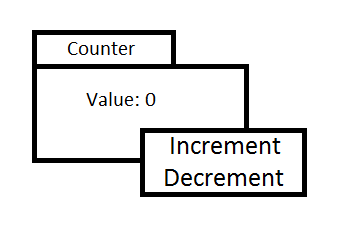
\includegraphics[scale=0.85]{counter.png}
\caption{Kuva CounterView -Näkymästä \parencite{krasner_desc}}
\end{figure}

Seuraavaksi esitellään Dortmundin yliopistossa kirjoitettu yksinkertainen esimerkkiohjelma Smalltalkilla, siitä miten MVC:n toteutus tuodaan sovellukseen käytännössä. Ohjelmakoodi löytyy myös Krasnerin artikkelista \parencite[s. 20]{krasner_desc}. Ohjelmassa toteutetaan yksinkertainen laskuriohjelma, joka käyttää MVC-arkkitehtuuria toteutuksessaan. Ohjelmassa esitellään Mallina \emph{Counter} -luokka ja Näkymänä \emph{CounterView} -luokka. \emph{Counter} perii Mallin ominaisuudet ja
toimii ohjelmassa yksinkertaisen kokonaisluku-muuttujan ylläpitäjänä. \emph{CounterView} perii Näkymän ominaisuudet ja esittää Mallin arvon ruudulla.
Ohjaimena toimii \emph{CounterController} -luokka, joka perii Ohjaimen käyttäytymisen. Ohjain tarjoaa sovellukselle painikkeet, joista voidaan vähentää
tai lisätä laskurin arvoa.


Määritellään ensiksi \emph{Counter} -luokka, joka peritään \emph{Model} -luokasta.
\begin{lstlisting}[language=Smalltalk]
Model subclass: #Counter
	instanceVariableNames: 'value'
	classVariableNames: ''
	poolDictionaries: ''
  	category: 'Demo-Counter'
\end{lstlisting}
Seuraavaksi määritellään \emph{Counter}-luokalle metodeita, jotka määrävät
laskuriarvon alustamisen sekä muokkaamisen.
\begin{lstlisting}[language=Smalltalk]
Counter methods For: 'Initialize-release'
Initialize
	"Aseta alkuarvoksi 0"
	self value: 0
Counter methodsFor: 'accessing'
value
	"Palauta Mallin arvo"
   	^value
value: aNumber
	"Aseta Mallin arvo"
	value <- aNumber.
	self changed "to update displayed value"
Counter methodsFor: 'operations'
decrement
	"Vähennä Mallin arvoa yhdellä."
	self value: value -1
Increment
	"Lisää Mallin arvoa yhdellä."
	self value: value + 1
\end{lstlisting}
Lisätään luokkaan metodi, jolla itse luokasta saadaan muodostettua instanssi.
\begin{lstlisting}[language=Smalltalk]
Counter class methodsFor: 'instance creation'
new
	"Palauta uusi instanssi luokasta"
	^super new initialize
\end{lstlisting}
Seuraavaksi määritellään Ohjain (\emph{CounterController}), joka peritään
\emph{Controller} luokasta. Luodaan myös Ohjaimelle metodit, joiden avulla
ohjataan Mallia sekä Näkymää. Metodeissa toteutetaan valikko, joka tarjoaa
mahdollisuuden joko vähentää tai lisätä laskurin arvoa. Kaikki \emph{CounterController} -luokassa käytetyt
määrittelemättömät muuttujat peritään yläluokasta.
\begin{lstlisting}[language=Smalltalk]
Mouse MenuController subclass: #CounterControIler
	instanceVariableNames: ' '
  	classVariableNames: ' '
  	poolDictionaries: ' '
  	category: 'Demo-Counter'
CounterController methodsFor: 'initialize-release'
initialize
	"Alusta valikko, jossa on mahdollisuus vähentää tai 
        lisätä Mallin arvoa"
  	super initialize.
  	Self yellowButtonMenu: (PopUpMenu labels: 
                                  'Increment\Decrement' withCRs)
  	yellowButtonMessages: #(increment decrement)
CounterController methodsFor: 'menu messages'
decrement
	"Vähennä Mallin arvoa yhdellä."
 	self model decrement
increment
	"Lisää Mallin arvoa yhdellä"
	self model increment
CounterController methodsFor: 'control defaults'
isControlActlve
	"Ota hallinta kun sinistä nappia ei paineta"
	^super isControlActive & sensor blueButtonPressed not
\end{lstlisting}
Määrätään Näkymä (\emph{CounterView}), joka peritään \emph{View} -yläluokasta. Määrätään
myös Näkymälle metodit, joiden avulla näytetään Mallin tila ruudulla.
\begin{lstlisting}[language=Smalltalk]
View subclass: #Counterview
	instanceVariableNames: ''
	classVariableNames: ''
	poolDictionaries: ''
	category: 'Demo-Counter'

CounterView methodsFor: 'displaying'
displayView
	"Näytä Mallin arvo Näkymässä"
	| box pos displayText |
	box := self insetDisplayBox.
	"Asettele teksti Näkymään. Asettelu ei
	 ole tutkielman kannalta oleellista."
	pos := box origin + (4 @ (box extent y / 3)).
	displayText := ('value:', self model value printString)
					asDisplayText.
	displayText displayAt: pos
\end{lstlisting}
Määritellään \emph{update} -metodi, jotta Näkymä pystyy päivittämään itsensä. Metodia kutsutaan
yleensä Mallin tilan muuttuessa.
\begin{lstlisting}[language=Smalltalk]
CounterView methodsFor: 'updating'
update: aParameter
  "Yksinkertaisesti päivitä näyttö uudestaan"
  self display
\end{lstlisting}
Luodaan myös metodi, joka palauttaa Näkymään liitetyn Ohjaimen.
\begin{lstlisting}[language=Smalltalk]
CounterView methodsFor: 'controller access'
defaultControllerClass
	"Palauta Näkymään rekisteröity Ohjain"
	^CounterController
\end{lstlisting}
Lopuksi tarvitaan metodi, joka luo uuden Näkymän sekä rekisteröi Mallin ja Ohjaimen itseensä. Näkymä näyttää ruudulta
samalta kuin kuvassa 2.
\begin{lstlisting}[language=Smalltalk]
CounterView class methodsFor: 'instance creation'
open
	"Avaa Näkymän uudelle laskurisovellukselle. Tässä 
	metodissa nähdään kuinka Näkymä huolehtii Mallin 
	rekisteröinnistä sekä nähdään kuinka näkymiä voi 
	olla useita sisäkkäin."
	| aCounterView topView |
	"Luo laskurinäkymälle uusi Näkymä, joka näyttää 
	laskurin arvon"
	aCounterView := CounterView new
	"Asetetaan Malliksi Counter -luokan instanssi"
	model: Counter new.
	aCounterView borderWidth: 2.
	aCounterView insideColor: Form white.
	"Asetetaan ylimmäksi Näkymäksi StandardSystemView 
	-luokan instanssi, joka vastaa perinteistä
ikkunointimallia"
	topView := StandardSystemView new
		label: 'Counter'.
	topView minimumSize: 80@40.
	"Lisätään edellä luotu laskurinäkymä ylänäkymän 
	alanäkymäksi"
	topView addSubView: aCounterView.
	"Käynnistetään Ohjain"
	topView controller open
\end{lstlisting}


\section{Vaatimukset}
Pyramidin sekä Djangon sovellusarkkitehtuuri on toteutettu käyttäen pohjana MVC"-arkkitehtuuria. Tämä ei kuitenkaan tarkoita sitä, että ne toteuttaisivat MVC:n teknisesti sellaisena kuin esimerkiksi Krasner \parencite{krasner_desc} ja Reenskaug \parencite{reenskaug_tools} määrittelee. Tärkeimpänä vaatimuksena MVC:n toteutukselle on se, että Näkymä ja Ohjain luovat rajapinnan, jonka kautta käyttäjä keskustelee Mallin kanssa. Malli ei saa olla suorassa yhteydessä käyttäjään \parencite[s. 10]{reenskaug_tools}. Mallin tulee olla riippumaton Näkymästä ja Ohjaimesta. Sen tulee myös hallita sovelluksen tilaa sekä pystyä antamaan informaatiota sovelluksen tilasta \parencite{burbeck}. Näkymän on keskusteltava Mallin kanssa sekä hoitaa Mallilta saadun datan graafinen näyttäminen \parencite[s.1]{reenskaug_orig}. Ohjain puolestaan ottaa vastaan syötteitä ja lähettää viestejä tämän perusteella Näkymälle ja Mallille \parencite{burbeck}.

Vaikka MVC:tä ei ole tarkoitettu alun perin web-sovelluksiin, voivat ne hyötyä MVC:n arkkitehtuurista. Suurin ongelma MVC:n käyttämisessä web-sovelluskehyksissä on palvelimen (palvelin) ja asiakkaan (client) välinen ositus. Näkymä näytetään aina asiakkaan selaimessa sen omalla päätelaitteella. Malli ja Ohjain taas voivat olla pilkottu teoriassa miten vain asiakkaan ja palvelimen välillä. Web-sovelluksissa kehittäjä pakotetaan pilkkomaan sovellus. MVC:n tulee olla riippumaton pilkkomisesta. Pilkkomisen ei tule määrittää sovelluksen arkkitehtuuria \parencite{ibm_watson}. Sen yhteydessä tulee myös mahdollistaa kaksisuuntainen kommunikaatio palvelimen ja selaimen välille. Reenskaugin mukaan Mallin tulee pystyä lähettämään itsestään muutosviestejä siihen kytketyille komponenteille. Tässä tapauksessa web-sovelluskehyksissä toteutetun Mallin tulee lähettää viestejä suoraan Näkymille ja Ohjaimille \parencite{reenskaug_tools}. 

\chapter{Sovelluskehykset}
Sovelluskehykset ovat suosittuja, koska ne tarjoavat uudelleenkäytettäviä ratkaisuja erilaisiin ongelmiin sovelluskehityksessä \parencite{towards_framework}. Toimialueesta riippumatta sovelluskehyksiä tulisi käyttää hyväksi kirjottaessa monimutkaisia sovelluksia. Sovelluskehys tuo sovellukseen tason, jossa sovelluksen osat on abstrahoitu erilaisilla luokilla sekä rajapinnoilla, joita voidaan käyttää uudelleen sovelluksen eri osissa. Sovelluskehys ei ole vain kokoelma rajapintoja ja kirjastoja\parencite{towards_framework}. Tärkein ero sovelluskehyksen ja kirjaston välillä on se, että kirjaston ohjelmakoodi kutsutaan aina
kehittäjän toimesta. Sovelluskehyksessä taas kehittäjän ohjelmakoodia kutsutaan aina sovelluskehyksen toimesta \parencite{pyramid_intr}.

Sovelluskehys ei myöskään generoi koodia. Se käyttää erilaisia komponentteja ja kirjastoja luodakseen infrastruktuurin, jonka päälle voidaan rakentaa sovelluksia sovelluskehyksen ehdoilla. Sovelluskehyksen käyttäminen myös rajoittaa sovelluksen rakennetta ja pakottaa sovelluksen toteuttamaan asioita tietyin ehdoin. Rajoitusten ansiosta sovelluskehittäjä voi keskittyä toimialueeseen liittyviin ongelmiin välittämättä koko sovelluksen yksityiskohtaisesta toteutuksesta
Olio-ohjelmoinnin etuna on olioiden uudelleenkäyttäminen eri järjestelmien kesken. On kuitenkin huomattu olioiden olevan usein hyvin yksinkertaisia ja ne on suunniteltu erityisesti yhden järjestelmän näkökulmasta. Tästä syystä niiden uudelleenkirjoitus on usein nopeampaa kuin olemassa olevien olioiden omaksuminen. Olioiden uudelleenkäytettävyyden on todettu parhaiten toimivan sovelluskehysten tuomien abstraktioiden kautta. Sovelluskehys on geneerinen rakennuspohja, jota laajennetaan luomaan vaatimuksien mukainen sovellus \parencite[s. 431]{Sommerville}. Schmidt \parencite{frameworks} määrittelee sovelluskehyksen seuraavasti: "Sovelluskehys on kokoelma ohjelmisto-artefakteja kuten luokkia, olioita ja erilaisia komponentteja, jotka yhdessä tarjoavat uudelleenkäytettävän arkkitehtuurin samaan perheeseen kuuluvien ohjelmistojen toteuttamiseksi".

Sovelluskehykset tarjoavat geneerisiä työkaluja sekä ominaisuuksia, joita voidaan käyttää samantyyppisissä sovelluksissa. Esimerkiksi käyttöliittymälle tarkoitettu sovelluskehys sisältää työkaluja erilaisten näkymien toteuttamiseen. Ohjelmistokehittäjän vastuulle jätetään sovelluskehyksen tarjoamien ominaisuuksien laajentaminen sovelluksen vaatimusten mukaiseksi. Sovelluskehys suunnitellaan siten, että se toimii sovelluksen runkona ja sen arkkitehtuuri toteutetaan luokkien sekä olioiden kommunikaation pohjalta. Luokkia käytetään usein suoraan sellaisenaan tai niitä laajennetaan käyttämällä erilaisia ohjelmointikielen ominaisuuksia kuten esimerkiksi perintää. Sovelluskehykset rakennetaan lähes aina olio-ohjelmointia käyttäen ja ne ovat hyvin usein riippuvaisia tietystä ohjelmointikielestä. Sovelluskehyksiä on tarjolla lähes jokaiselle yleisimmälle olio-ohjelmointiparadigman toteuttavalle ohjelmointikielelle. Sovelluskehykset voivat myös sisältää useita pienempiä sovelluskehyksiä, joissa jokainen on suunniteltu toteuttamaan jonkun tietyn osan sovelluksesta. Sovelluskehystä voidaan käyttää luomaan koko sovellus tai vain tiettyjä osia sovelluksesta kuten esimerkiksi graafisen käyttöliittymän \parencite[s. 431]{Sommerville}.

Schmidt \parencite{frameworks} jakaa sovelluskehyksien arkkitehtuurit kolmeen luokkaan:


\begin{desclist}
\item[Infrastruktuuri-sovelluskehykset (System infrastructure frameworks)] tarjoavat työkaluja hallitsemaan järjestelmätason sovelluksia sekä niiden kommunikaatiota keskenään. Tällaisia ovat esimerkiksi erilaiset kääntäjät ja järjestelmätason käyttöliittymät. 
\item[Integraatio-sovelluskehykset (Middleware integration frameworks)] sisältää kokoelman standardeja sekä luokkia, jotka auttavat komponenttien väliseen kommunikaatioon sekä tiedonsiirtoon. Tällaisia ovat esimerkiksi Microsoftin .NET ja EJB (Enterprise Java Beans). 
\item[Liiketoiminta-sovelluskehykset (Enterprise application frameworks)] keskittyvät tiettyjen sovelluksien osa-alueisiin, kuten esimerkiksi telekommunikaation tai laskutusjärjestelmien toteutukseen. Ne ovat erityisesti suunnattuja loppukäyttäjälle.
\end{desclist}

Web-sovelluskehykset ovat nykyaikana yksi tärkeimpiä sovelluskehyksien alalajeja. Web-sovelluskehyksiä, jotka tarjoavat työkaluja dynaamisten web-sovellusten toteuttamiseen, on tarjolla paljon. Yleisesti näiden sovelluskehysten arkkitehtuurina on käytetty MVC-arkkitehtuuria. Tämän takia monet web-sovelluskehykset mielletään MVC-sovelluskehyksiksi, vaikka MVC esiteltiinkin 80-luvulla eri tarkoitukseen. Sovelluskehykset voivat koostua useista arkkitehtuurimalleista. Esimerkiksi MVC-sovelluskehys koostuu Tarkkailumallista (Observer Pattern), Strategiamallista (Strategy Pattern), Yhdistelmämallista sekä monista muista, jotka esitellään (Design Patterns: Elements of Reusable Object-Oriented Software) -kirjassa \parencite{design_patterns}. Vaikka jokainen web-sovelluskehys on toteutettu hieman erilaisella tavalla, Sommerville esittelee viisi perusominaisuutta, jotka yleensä löytyvät web-sovelluskehyksistä:

\begin{desclist}
\item[Tietoturva] Sovelluskehykset tarjoavat luokkia auttamaan käyttäjänhallinnan toteutuksessa, siten että sovellukseen voidaan luoda erilaisia rajoituksia käyttäjille. 
\item[Dynaamisten web-sivut] Työkalut luoda sivupohjia (template), joiden pohjalta voidaan data näyttää eri tavoilla selaimelle.
\item[Tietokantatuki] Työkalut tietokantoihin yhdistämiseen ja niiden käyttöön. Web-sovelluskehykset eivät yleensä sisällä tietokantaa, mutta ne on usein rakennettu tietyn tietokantatyypin pohjalta. Niillä on erilaisia luokkia, joilla voidaan abstrahoida tietokannan käyttö.
\item[Session-hallinta] työkalut sessioiden luontiin ja hallintaan.
\item[Interaktiivisuus] Mahdollisuus toteuttaa entistä interaktiivisempia sovelluksia käyttäjille. 
\end{desclist}

Sovelluskehystä laajennettaessa ei sovelluskehyksen ohjelmakoodia muuteta, vaan sovellukseen lisätään luokkia, jotka perivät sovelluskehyksen määrittelemiä ominaisuuksia luokkatasolla. Lisäksi voidaan määritellä takaisinkutsuja (callbacks). Takaisinkutsuja voidaan viedä eteenpäin toiselle ohjelmakoodille kutsuttavaksi. Takaisinkutsuja ajetaan vastauksena ennalta määrätyille operaatiolle, jotka sovelluskehys tunnistaa. Sovelluskehykseen luodut toiminnot ovat vastuussa sovelluksen kokonaisuudesta, siten että ne kutsuvat sovelluskehyksen käyttäjän määrittelemiä toiminnallisuuksia. Sovelluskehykseen toteutetut oliot ovat vastuussa erilaisten tapahtumien hallinnoinnista ja välittävät näitä tapahtumia edelleen käyttäjän tekemälle sovelluskoodille. Tällaisia toimintoja kutsutaan koukku-metodeiksi (hook method). Niiden tehtävä voi olla esimerkiksi toteuttaa jokin tietty toiminallisuus aina silloin, kun tietokantaan tehdään kirjoitusoperaatioita \parencite[s. 433]{Sommerville}. 


\begin{figure}[h]
\centering
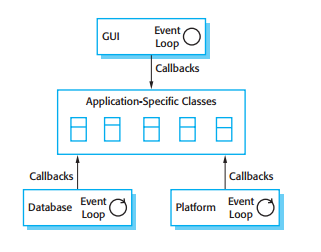
\includegraphics[scale=0.85]{frameworks.png}
\caption{Esimerkki sovelluksen toimintojen suhteesta sovelluskehyksen takaisinkutsuihin. Sovelluskehyksellä voi olla esimerkiksi metodi, joka hallitsee hiiren tapahtumia. Metodi kutsuu koukku-metodia, joka tulee konfiguroida kutsumaan oikeita metodeja sovelluksesta, jossa hiiren tapahtumat käsitellään \parencite[s.434]{Sommerville}.}
\end{figure}

Sovelluskehyksien avulla rakennetut sovellukset voivat toimia uudelleenkäytettävinä pohjina jollekin tietylle liiketoiminta-alueella tai sovellusperheelle. Koska näissä sovelluksissa on käytetty jotain tiettyä sovelluskehystä, voidaan sovelluksesta luoda monia instansseja, jotka palvelevat jotain tiettyjä alueita liiketoiminnassa. Koska kaikki sovellukset jakavat saman sovelluskehyksen tavan toteuttaa asioita, on uusien sovellusperheen jäsenten luonti usein hyvin suoraviivaista. Tämä mahdollistetaan ylikirjoittamalla pohjasovellukseen luokkia ja metodeja, joita voidaan muokata ylikirjoittamalla se taas uudessa sovelluksessa. Osa näistä luokista voi olla ylimmällä tasolla peritty suoraan sovelluskehyksestä. Sovelluskehykset ovat kuitenkin yleensä hyvin geneerisiä kuin eri
liiketoiminta-alueiden sovellukset. Web-pohjaisia sovelluskehyksiä voidaan esimerkiksi käyttää toteuttamaan asiakaspalvelulle tarkoitettuja web-sovelluksia. 

Sovelluskehykset ovat tehokkaita sovelluksien uudelleenkäytössä, mutta ne ovat myös kalliita tuoda sovelluskehitykseen mukaan. Sovelluskehykset ovat usein hyvin monimutkaisia ja niiden omaksuminen voi kestää kuukausia. Virheiden etsintä on sovelluskehyksien pohjalta tehdyissä sovelluksissa haastavaa, koska ohjelmoijan tulee ymmärtää, millä tavalla sovelluskehys toimii. Lisäksi voi olla vaikeaa valita oikea sovelluskehys monien joukosta. 

\chapter{Web-sovelluskehykset \& MVC}
Web-sovelluskehykset ovat sovelluskehyksiä, jotka tarjoavat ratkaisuja helpottamaan web-sovellusten toteuttamista. Web-sovelluskehyksissä käyttöliittymä näytetään käyttäjille selaimen välityksellä. Sovellus ajetaan joko palvelimella tai suoraan käyttäjän selaimessa. Sovellus määrittää käyttöliittymän sivujen järjestyksen, sisällön sekä mahdollisten toimintojen esittämisen käyttäjälle, jonka kautta käyttäjä voi vaikuttaa palvelimella sijaitsevaan sovellukseen \parencite{vosloo}. 

Yleisimmät teknologiat mitä web-sovelluskehykset tarjoavat ovat erilaiset rajapinnat tietokannalle, sivupohjamoottori sekä mahdollisuus käsitellä HTTP-pyyntöjä ohjelmakoodissa. Tietokantarajapinnalla tuodaan sovelluskehitykseen taso, jonka avulla helpotetaan kommunikointia tietokannan kanssa. Yleisimmin käytetty ohjelmointitekniikka tähän on ORM (Object-Relational-Mapping), jolla muunnetaan dataa tietokannan ja ohjelmakoodin välillä. Ohjelmoijalle tämä näkyy ns. virtuaalisena oliotietokantana, jonka avulla voidaan lukea sekä muokata tietokantaa kutsuilla ohjelmakoodista. Tällöin suoria kyselyitä tietokantaan ei tarvita \parencite{Ghandeharizadeh}. Seuraavassa esimerkissä esitellään, miten Djangon ORM:ia käytetään.


\begin{lstlisting}[language=Python]
from django.db import models

class Blog(models.Model):
    name = models.CharField(max_length=100)
    tagline = models.TextField()
\end{lstlisting}

\begin{lstlisting}[language=Python]
from blog.models import Blog

b = Blog(name='Beatles Blog', tagline='All the latest Beatles news.')
b.save()
\end{lstlisting}

Esimerkissä luodaan luokka, jolla määritellään taulu SQL-tietokantaan. Model-luokasta periminen mahdollistaa luokasta luotujen instanssien tallentumisen tauluun. Lisäksi
luokalle voidaan määrittää attribuutteja, jotka käyttävät Djangon tarjoamia kenttiä. Kentät vastaavat tietokannassa olevia datatyyppejä. Lopullinen tallentuminen
tapahtuu kutsumalla instanssin save-metodia.


\begin{lstlisting}[language=Python]
beatles_blog = Blog.objects.get(name="Beatles Blog")
\end{lstlisting}

Yllä oleva rivi hoitaa kyselyn nimen perusteella \emph{Blog} -nimisestä taulusta, luo sen kenttien perusteella instanssin Blog -luokasta ja tallentaa sen muuttujan arvoksi.
Sivupohjamoottori on teknologia HTML-sivujen tuottamiseen, jolla generoidaan dynaamisia HTML-sivuja yhdistämällä ohjelmalogiikkaa sekä HTML-kieltä. Alla on esitelty Jinja2-kieli, jota käytetään sivupohjakielenä Flask-sovelluskehyksessä.

\begin{lstlisting}[language=Smalltalk]
<title></title>
<ul>
  
	<li><a href="{{ user.url }}">{{ user.username }}</a></li>
  
</ul>
\end{lstlisting}


Yllä esitellyssä esimerkissä luodaan HTML-sivu, jossa tulostetaan otsikko sekä lista URL-osoitteita sekä käyttäjänimiä jokaista käyttäjää kohden \parencite{jinja}.

Web-sovelluskehykset voidaan jakaa palvelinpohjaisiin ja selainpohjaisiin sovelluskehyksiin. Palvelinpohjaisissa web-sovelluskehyksissä sovelluksen tilaa hallitaan palvelimen puolella. Tuolloin käyttöliittymää perustuu tilaan, mikä on sillä hetkellä palvelimen puolella. Selainpohjaisissa sovelluskehyksissä sisältö muuttuu selaimen sisällä käyttäjän päässä \parencite{vosloo}. Tässä tutkielmassa käsiteltävät sovelluskehykset ovat Pythonilla toteutettuja palvelinpohjaisia sovelluskehyksiä. Käsiteltävät kehykset ovat Django, Pyramid ja Tornado. Django on käsiteltävistä sovelluskehyksistä kaikkein monoliittisin ja tarjoaa eniten ominaisuuksia valmiiksi asennettuna. Pyramidissa taas on vähemmän ominaisuuksia suoraan asennettuna, jonka kautta se pyrkii antamaan käyttäjälle enemmän valinnanvaraa erilaisten teknologioiden valitsemiseen. Tornado taas on sovelluskehys, joka tarjoaa kaikkein vähiten työkaluja web-kehitykseen. Sovelluskehysten koko kertoo niiden toteutuksesta: Django (1.11) 31 megabittiä, Pyramid (1.5.3) 5.6 megabittiä ja Tornado (4.5.2) 3.1 megatavua. Sovelluskehysten koot tarkastettiin komentoriviltä käyttäen linuxin du -työkalua (Disk Usage). Djangoa ja Pyramidia voidaan laajentaa erilaisilla laajennoksilla, mutta Tornadoon ei ole tarjolla laajennoksia. 

\section{Pyramid}
Pyramid on Python-pohjainen web-sovelluskehys, jonka tehtävänä on helpottaa web-kehitystä tarjoamalla
kehittäjälle valmiita työkaluja avuksi kehitykseen. Pyramid on suunniteltu siten, että kehittäjän ei tarvitse tietää suuria määriä erilaisia malleja ja tekniikoita pystyäkseen tuottamaan web-sovelluksia. Se ei myöskään pakota käyttämään kehityksessä mitään erityistä tekniikkaa, vaan pyrkii olemaan mahdollisimman yksinkertainen ja helposti laajennettavissa erilaisiin käyttötarkoituksiin. Laajentamisella tarkoitetaan erilaisten lisäosien liittämistä Pyramidiin. Yksinkertaisuuden ja minimaalisuuden ansiosta se on myös nopeampi kuin monet muut Python-pohjaiset web-sovelluskehykset. Tämä johtuu Pyramidin poikkeuksellisen pienestä kutsupinosta ajamisen aikana \parencite{pyramid_intr}. 

Pyramid sai alkunsa Pylons-projektista syyskuussa vuonna 2005, jolloin jo yli 30 Python-sovelluskehystä kilpaili käyttäjistä. Ben Bangert ja James Gardner alkoivat yhdessä kehittää sovelluskehystä, josta tuli lopulta Pylons. Alunperin Pylons oli
muokattu Myghty Python Templating Framework:n pohjalta tarjotakseen MVC-pohjaisen web-sovelluskehyksen. Myghty -sovelluskehystä ajettiin mod\_pythonin päällä, mutta Pylonsin pyrkimys oli käyttää WSGI:tä hyödyntämään joustavaa komponenttipohjaista lähestymistapaa web-sovelluksissa \parencite{pylons_history}. Pylons projektin tarkoituksena ei ole keskittyä yhden yksittäisen web-sovelluskehyksen kehittämiseen vaan tarjota kokoelma erilaisia teknologioita \parencite{pylons_about}. Vuonna 2008 Pyramid tunnettiin nimellä repoze.bfg. Joulukuun alussa tapahtui ohjelmakoodin uudelleen nimeäminen ja ominaisuuksien lisääminen sekä poistaminen \parencite{pyramid_about}.

Koska Pyramid pyrkii tarjoamaan vain välttämättömimmät työkalut web"-sovelluksien kehitykseen, sen kehittäjät
ovat päätyneet web-kehityksessä neljään yleisimpään ongelmaan ja tarjoavat niihin ratkaisun Pyramidissa:


\begin{description}
\item [URL Mapping] -\ URL:ien liittäminen ohjelmakoodiin.
\item[Template] -\ Tuodaan sovelluksen näkymä selaimelle käyttäen sivupohjia, jolla määrätään näkymän rakenne. Sivupohja sisältää usein HTML:n mukana tuotuja loogisia ilmaisuja, joiden perusteella sivupohjamoottori rakentaa HTML-sivun selaimelle. Sivupohjan avulla pystytään erottamaan käyttöliittymä sovelluslogiikasta tehokkaasti.
\item[Security] -\ Perinteiset tietoturvaongelmat tulee olla ratkaistuna valmiiksi jo sovelluskehyksessä. Tämä ei kuitenkaan tarkoita sitä, että kehittäjä voisi täysin unohtaa tietoturvan merkityksen.
\item[Static Assets] -\ Staattisien resurssien jakaminen niille tarkoitettuihin paikkoihin tiedostorakenteessa.
\end{description}
Yllä määriteltyjen neljän ongelman lisäksi Pyramid tarjoaa lisäosien kautta monia erilaisia työkaluja, joiden avulla pystytään laajentamaan sen ominaisuuksia \parencite{pyramid_intr}. Tutkielman aiheen rajauksen vuoksi ei kuitenkaan


\section{Django}
Djangon läpikäynnissä joudutaan turvautumaan täysin Djangon omiin dokumentaatioihin, jotka löytyvät Djangon web-sivulta. Django on web-sovelluskehys, joka sai alkunsa kehitysryhmässä Kansaksen osavaltiossa Yhdysvalloissa 2003, kun web-kehittäjät Adrian Holovaty ja Simon Willison alkoivat käyttää Pythonia web-kehityksessä. The World Online -ryhmä (WO), joka oli vastuussa muutamasta paikallisesta uutissivustosta, menestyivät ympäristössä, jossa oli tiukat aikarajat. Journalistit vaativat ominaisuuksien ja kokonaisten sovelluksien valmistumista muutamassa päivässä ja joskus jopa tunneissa. Holovaty ja Willison kehittivät web-sovelluskehyksen, jonka avulla he pystyivät vastaamaan journalistisen ympäristön haasteisiin. Kesällä 2005 he saivat kehitettyä sovelluskehyksen siten, että se oli käytössä suurimmassa osassa World Onlinen sivustoja. Tuolloin mukaan kehitykseen tuli Jacob Kaplan-Moss. Kehittäjät päättivät julkaista heinäkuussa 2005 sovelluskehyksen nimellä Django jazz-kitaristi Django Reinhardtin mukaan \parencite{django_history}.

Django tarjoaa samat välttämättömät työkalut kuin Pyramidissa. Se tarjoaa myös ylläpitäjille suunnatun työkalun, josta voidaan hallita sovellusta käyttöliittymätasolta. Lisäksi se tarjoaa lomaketyökalut, käyttäjätasoisen varmentamisen sekä tietokanta-abstrahoinnin. Tietokanta-abstraktiolla tarkoitetaan sisäänrakennettua virtuaalista ympäristöä tuomaan yhteys tietokantaan olio-ohjelmoinnin kautta (Object-relational mapping)\parencite{djangobook}. Siinä missä Pyramid pyrkii tarjoamaan kehittäjille valinnanvaraa erilaisten komponenttien suhteen, Django tarjoaa kokonaisvaltaisen ratkaisun sisältäen kaikki tarvittavat työkalut web-sovellusten rakentamiseen. Djangoon on tarjolla myös paljon erilaisia paketteja täydentämään sitä. 


\section{Tornado}
Tornado on Python-pohjainen web-sovelluskehys, joka pystyy skaalautumaan kymmenille tuhansille yhtäaikaisille yhteyksille. Se käyttää asynkronista siirräntää (asynchronous non-blocking I/O) sekä mahdollistaa web-sokettejen käytön \parencite{tornado}. Siirräntä tarkoittaa tässä yhteydessä luku- ja kirjoitusoperaatioita levyllä. Suurella kuormalla toimivat synkroniset TCP/IP-sovellukset voivat jättää useita syklejä prosessorin laskennasta väliin, joka johtuu siirrännän hitaudesta. Nämä syklit voitaisiin käyttää sovelluksen koodin ajamiseen. Mitä enemmän pyyntöjä tulee samanaikaisesti, sitä enemmän prosessorin syklejä jää väliin ja järjestelmään tulee ylimääräistä kuormaa. Siirrännät ovat paljon hitaampia kuin prosessorin laskentateho. Asynkronisessa siirrännässä pyyntöjä voidaan ottaa vastaan käsiteltäväksi, vaikka edellistä pyyntöä ei ole vielä suoritettu loppuun \parencite[s. 1]{async}. Tornado ei toteuta MVC-mallia, vaan tarjoaa vapaammat kädet kehittäjälle toteuttaa haluamansa arkkitehtuuri. 


\section{MVC \& Pyramid}
Pyramidin kehittäjien dokumenteissa esitellään MVC-kehyksenä, mutta samalla myös kyseenalaistetaan tämä väite. Erityisesti Mallin ja Ohjaimen määritelmä puuttuu \parencite{pyramid_intr}. Tässä
osiossa käsitellään Pyramidia MVC:n näkökulmasta. Tarkastelua varten toteutetaan Pyramidilla vastaava laskuri-sovellus kuin Krasnerin julkaisussa käyttäen Pyramidin tarjoamia ominaisuuksia \parencite{krasner_desc}. Sovellus rajataan käyttämään SQL-tietokantaa Mallin datan tallennukseen sekä \emph{URL dispatch} -tekniikkaa \parencite{urldispatch}. Sovelluksen pohjalta tarkastellaan MVC:n kannalta kolmea oleellisinta tiedostoa: \emph{views.py}, \emph{models.py} ja \emph{template.pt}. Näin tutkielman tarkastelu pystytään rajaamaan mahdollisimman pienelle alueelle, jolloin tutkielma on helpompi keskittää tarkastelemaan yksittäistä tekniikkaa.

Tässä osiossa tarkastellaan Pyramid-sovelluksen tiedostoja sekä niiden sisältöjä MVC-komponenttien näkökulmasta. Erityisesti keskitytään Ohjaimen ja Näkymän toteutukseen. Samalla tutkitaan, voidaanko Pyramid havaintojen perusteella luokitella MVC:n toteuttavaksi sovelluskehykseksi.
Koska Pyramidissa MVC:n määrittely on hyvin epävakaalla pohjalla, tulee tehdä selväksi, mitä ominaisuuksia komponenteilta vaaditaan. Esimerkiksi \emph{views.py} ja \emph{template.pt} -tiedostot ovat tarkoitettu toimimaan yhdessä näkymänä, jolloin Ohjaimen toteuttamat tehtävät sisällytettäisiin Näkymään. MVC:tä tutkiessa täytyy sovelluksen komponentit kuitenkin jakaa kolmeen osaan. Tiedosto \emph{views.py}
sisältää paljon Ohjaimelle yhteisiä piirteitä, joten se erottuu selvästi \emph{template.pt} -tiedostosta. Tutkielmassa oletetaan, että \emph{models.py} sisältää Mallin, \emph{views.py} Ohjaimen ja \emph{template.pt} Näkymän.

\lstset{
  literate={ö}{{\"o}}1
           {ä}{{\"a}}1,
xleftmargin=30pt,
escapeinside={/*@}{@*/},
backgroundcolor=\color{light-gray}
}
\lstset{numbers=left}
\begin{lstlisting}[language=Python]
# Tiedosto: models.py
class Counter(Base):
    __tablename__ = 'counter'

    # Asetetaan Mallille atribuutit, jotka
    # vastaavat Mallin tilasta.
    id = Column(Integer, primary_key=True)
    name = Column(Unicode(255), unique=True)
    value = Column(Integer)

    # Määritellään luokalle konstruktori,
    # joka saa parametreiksi nimen ja alkuarvon.
    def __init__(self, name, value):
        self.name = name
        self.value = value

    def increment(self):
        self.value += 1

    def decrement(self):
        self.value -= 1

# Luodaan instanssi Mallista ja rekisteröidään 
# se sovellukseen.
def populate():
    session = DBSession()
    model = Counter(name=u'counter', value=0)
    session.add(model)
\end{lstlisting}
\emph{Models.py} -tiedosto sisältää Malliin liittyvän ohjelmakoodin. Jokaiselle Mallille luodaan aina oma luokkansa, jossa määritellään Mallin ominaisuudet. Malli rekisteröidään \emph{populate} -funktion kautta, jota kutsutaan Pyramidin toimesta.
Ohjelmakoodista nähdään, että Malli ei luo minkäänlaista riippuvuutta Näkymään tai Ohjaimeen. Se myös pitää huolen datan käsittelystä. Malli on siis Pyramidissa itsenäinen komponentti, joka huolehtii sovelluksen tilasta. Tämän perusteella Malli toteutuu Pyramidissa MVC-arkkitehtuurin mukaisesti.
\emph{Views.py} -tiedostossa määritellään Näkymän ohjelmakoodi. Pyramidissa on konkreettisesti määritelty ohjelmakooditasolla vain Malli ja Näkymä.
Jokaista Näkymää kohden on oma funktio, joka ottaa vastaan \emph{request}-olion. Oliossa tuodaan sovellukselle kaikki tieto käyttäjästä ja sovelluksen viesteistä. Tämän perusteella tulkitaan \emph{request}-oliossa tuotu data käyttäjän syötteiksi.
Vaikka \emph{views.py} nimetään Pyramidissa Näkymäksi, on se toteutukseltaan hyvin lähellä Ohjainta. Tästä syystä tarkastellaan funktion toteutusta mahdollisena Ohjaimena. Tästä eteenpäin puhuttaessa Ohjaimesta Pyramidissa, tarkoitetaan sillä \emph{views.py} -tiedoston sisältämää funktiota.

\lstset{
  literate={ö}{{\"o}}1
           {ä}{{\"a}}1,
xleftmargin=30pt,
escapeinside={/*@}{@*/},
}
\begin{lstlisting}[language=Python]
# Tiedosto: views.py
@view_config(route_name='counter_view',
	renderer='templates/counter.pt')
def counter_view(request):
    dbsession = DBSession()

    # Rekisteröidään Malli.
    counter = dbsession.query(Counter).filter(
	Counter.name==u'counter').first()
    try:
        request.params['minus'].
        counter.decrement()
    except KeyError:
        pass

    try:
        request.params['plus']
        counter.increment()
    except KeyError:
        pass

    # Palautetaan laskurin arvo, joka tulkitaan
    # ja näytetään template.pt -tiedostssa
    return {'value': counter.value}
\end{lstlisting}
Määritellään funktiolle URL-osoite sekä liitetään siihen sivupohjatiedosto (2). Tämän jälkeen rekisteröidään Malli mukaan funktioon (8). Koska tarkastelemme funktiota Ohjaimena, voimme tulkita sivupohjan Näkymäksi. Tällöin funktioon rekisteröidään Malli sekä Näkymä, jolloin rekisteröinnin puolesta se toteuttaa Ohjaimelle tarkoitetut ominaisuudet MVC:ssä. Funktioon lisätään myös toiminto laskurin vähentämiselle. Mallin \emph{value} -arvoa muutetaan, kun request-oliosta löytyy tietty parametri. Funktio palauttaa paluuarvona Mallin arvon, joka tuodaan käsiteltäväksi sivupohjaan. Funktio siis ottaa vastaan syötteitä ja niiden perusteella lähettää viestejä Mallille ja Näkymälle. Tämän perusteella todetaan, että se täyttää rajauksessa määrätyt Ohjaimen ominaisuudet. 

Sivupohjassa yhdistetään HTML-merkkauskieli ja sovelluksen ohjelmakoodi. Tästä generoidaan HTML-sivu, joka näytetään selaimelle. Koska Malli sekä Ohjain on jo määritelty, täytyy selvittää täyttääkö sivupohja Näkymälle määritellyt ominaisuudet.
\begin{lstlisting}[language=Python]
<body>
<h1>${value}</h1>
<form action="./" method="get">
<button type="submit" name="plus" value="plus">
Increment </button>
<button type="submit" name="minus" value="minus"> 
Decrement </button>
</form>
</body>
\end{lstlisting}
Sivupohjassa luodaan lomake kahdelle painikkeelle, joista kumpikin lähettää lomakkeen eteenpäin \emph{counter\_view} -funktiolle. Lomakkeen tiedot tulevat funktiolle \emph{request}-oliossa, joka sisältää tässä tapauksessa \emph{plus}- tai \emph{minus}-parametrin riippuen siitä kumpaa painiketta on painettu. Lomakkeen tiedot lähetetään samaan osoitteeseen (3), mistä sitä on alun perin kutsuttukin. Eron tuo kuitenkin \emph{request}-oliossa tuodut parametrit. Otsikossa (2) tuodaan näkyviin laskurin sen hetkinen arvo, joka saadaan tietoon Ohjaimelta.

Sivupohjassa hoidetaan sovelluksen graafinen puoli, joten se vastaa ominaisuuksiltaan Näkymää. \\ Ongelmaksi muodostuu kuitenkin Näkymän ja Mallin välinen kommunikointi. Näkymä ei ole yhteydessä Malliin suoraan, vaan tarvitsee Ohjaimen kautta tiedon Mallin tilasta. Näkymä ei siis sellaisenaan toteuta sille asetettuja ominaisuuksia. \\

Alla olevassa kuvassa esitellään visuaalisesti miten laskurisovellus muodostaa HTML-sivun, kun käyttäjä painaa sivulla \emph{Increment} -painiketta. Kuvan
vaiheet toteutetaan numerojärjestyksessä alkaen ensimmäisestä.


\begin{figure}[h]
\centering
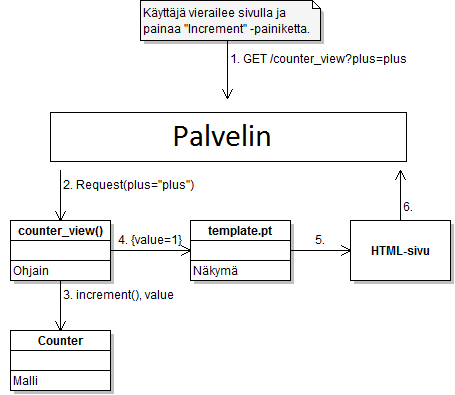
\includegraphics[scale=0.7]{laskurisovellus.png}
\caption{Laskurisovelluksen toiminta}
\end{figure}
\lstset{
  literate={ö}{{\"o}}1
           {ä}{{\"a}}1,
xleftmargin=30pt,
escapeinside={/*@}{@*/},
}

\begin{lstlisting}
/*@Palvelimelta pyydetään HTTP-protokollan mukaisesti sivua \emph{plus} -parametrilla.@*/
/*@Palvelin pyytää sovellukselta sivua. Parametri tuodaan sovellukselle \emph{request}-oliossa.@*/
/*@Ohjain käskee Mallia muuttamaan tilaansa ja pyytämään samalla tiedon muutoksen jälkeisestä arvosta.@*/
/*@Ohjain palauttaa Mallin arvon, joka käsitellään sivupohjassa.@*/
/*@Sivupohjassa generoidaan HTML-sivu, joka tuodaan palvelimelle vastauksena.@*/
\end{lstlisting}


\section{MVC \& Django}
Django luokitellaan MVC-arkkitehtuurin toteuttavaksi web-sovelluskehykseksi, mutta sen toteutus kuitenkin poikkeaa alkuperäisestä MVC-toteutuksesta samalla tavalla kuin Pyramidissa. Djangosta löytyvät samat tiedostot  ja luokat MVC:n toteuttamiselle, kuin Pyramidista. Siinä on vastaavasti \emph{models.py}, \emph{views.py} sekä \emph{template.html}. Näistä \emph{models.py} sisältää mallit, \emph{views.py} ohjaimet ja \emph{template.html} näkymät selaimelle. Tässä tutkielmassa  käytetään Djangon versiota 1.11. Seuraavaksi esitellään lyhesti Mallin, Näkymän sekä Ohjaimen toteutus Djangossa, jotka on myös esitelty Djangon dokumentaatiossa \parencite{django_docs}.

Mallin toteutetaan luomalla luokka, joka peritään \emph{models.Model} luokasta. Alla esitetyssä esimerkissä luodaan Malli, jolla voidaan tallentaa henkilön etu- ja sukunimi \parencite{django_model}.

\begin{lstlisting}[language=Python]
from django.db import models

class Person(models.Model):
    first_name = models.CharField(max_length=30)
    last_name = models.CharField(max_length=30)
\end{lstlisting}

Ohjaimen toiminta toteutuu Djangossa näkymien kautta vastaavasti kuin Pyramidissakin, koska näkymät käsittelevät pyyntöjä ja syötteitä, jotka tulevat selaimelta. Tästä syystä myös Ohjaimen määritelmä toteutuu sovelluskehyksessä määriteltyjen näkymien kautta \parencite{django_view}.

\begin{lstlisting}[language=Python]
from django.http import HttpResponse

def my_view(request):
    if request.method == 'GET':
        # <view logic>
        return HttpResponse('result')
\end{lstlisting}

Näkymät toteutetaan vastaavasti selaimelle käyttäen sivupohjia. Djangossa on sisäänrakennettuna oma sivupohjakieli, mutta se on hyvin samankaltainen esimerkiksi Jinja2 sivupohjakielen kanssa \parencite{django_template}.

\begin{lstlisting}[language=Python]


{{ section.title }}


<h1>{{ section.title }}</h1>


<h2>
  <a href="{{ story.get_absolute_url }}">
    {{ story.headline|upper }}
  </a>
</h2>
<p>{{ story.tease|truncatewords:"100" }}</p>


\end{lstlisting}


\section{Yhteenveto}
Malli sekä Ohjain toteutuvat Pyramidissa MVC:n mukaisesti yksittäisinä komponentteina, mutta kommunikaatio näiden välillä ei mene MVC:n mukaisesti. Malli on itsenäinen komponentti, jolla ei ole riippuvuutta Näkymään tai Ohjaimeen. Se myös huolehtii sovelluksen käsittelemästä datasta ja vastaa tarvittaviin pyyntöihin. Se ei kuitenkaan pysty kertomaan Ohjaimelle ja Näkymälle omista muutoksistaan, koska kaikki muutokset tulevat Näkymälle asti vastauksena vasta HTTP-pyynnön mukana. Ohjain taas huolehtii \emph{request}-oliossa tulevista syötteistä ja vaikuttaa Malliin sekä Näkymään. Näkymä toteuttaa sovelluksen graafisen näyttämisen selaimelle, mutta ei toteuta sille määrättyjä sääntöjä. MVC:ssä Näkymän tarkoitus on kommunikoida suoraan Mallin kanssa. Tämä ei kuitenkaan onnistu Pyramidissa, jossa Näkymä on yhteydessä vain Ohjaimeen. Pyramidin MVC toteutusta tarkastellessa tulee ottaa huomioon yksittäisten komponenttien toteutus sekä niiden välinen yhteistyö. Yksittäiset komponentit toteutuvat Pyramidissa MVC-arkkitehtuurin mukaisesti, mutta niiden välinen yhteistyö ei toteudu. Pyramidin MVC-komponenttien kommunikointi voidaan esittää käyttäen pohjana muokaten Krasnerin kommunikaatiomallia \parencite{krasner_desc}.
Alla esitellyssä kuvassa havainnollistetaan, kuinka Mallin ja Näkymän kommunikaatio puuttuu täysin ja kaikki data tuodaan Ohjaimen kautta. Lisäksi Malli ei pysty kommunikoimaan muutoksista suoraan Ohjaimelle ja Näkymälle vaan tarvitsee aina erillisen HTTP-pyynnön.

Djangossa määritellään MVC samalla tavalla kuin Pyramidissakin. Tästä syystä voidaan todeta, että vaikka MVC-komponenttien vaatimukset toteutuvat yksittäin, tulee samat ongelmat vastaan kuin Pyramidissakin. Kommunikaatiomalli on ristiriidassa MVC:n alkuperäisen toteutuksen kanssa, mikä johtuu HTTP:n päälle rakennetusta toteutuksesta. Lisäksi Näkymä ei kommunikoi suoraan Mallin kanssa, vaan kommunikaatio Mallille toteutetaan Ohjaimen kautta. 

\begin{figure}[h]
\centering/
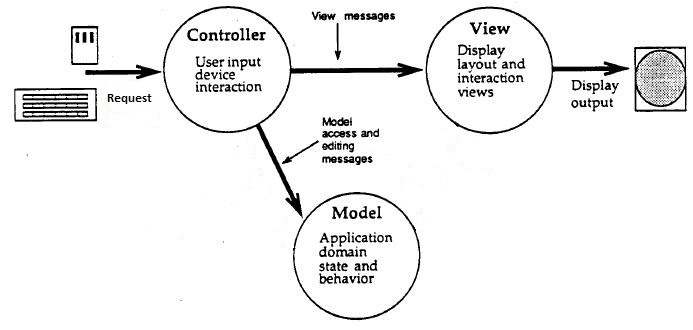
\includegraphics[scale=0.85]{pyramid_mvc.jpg}
\caption{Pyramidin kommunikointi MVC-komponenttien kesken. Kuva on muokattu Krasnerin esittelemästä kommunikointimallista \parencite{krasner_desc} }
\end{figure}
Yllä esitetyssä kommunikaatiomallissa Ohjain saa vastaan \emph{request}-olion, jossa tuodaan kaikki tarvittava tieto käyttäjästä. Tämän perusteella Ohjain käskee Mallia
sekä muuttujaa. Samalla se pyytää Mallilta tietoa sovelluksen tilasta ja välittää tiedon Näkymälle. Näkymä taas välittää Ohjaimen tuoman datan käyttäjälle graafisena.

Alun perin Pyramidin dokumentaatiossa kyseenalaistettiin Mallin sekä Ohjaimen toteutus \parencite{pyramid_intr}. Tutkimuksen pohjalta voidaan kuitenkin
todeta, että ongelmaksi ei muodostu yksittäisien komponenttien toteutus, vaan komponenttien välinen kommunikointi. Erityisesti Näkymän ja Mallin yhteistyö jää
kokonaan puuttumaan, jolloin saadaan ristiriita MVC:n alkuperäisen määritelmän kanssa \parencite[s. 1]{reenskaug_orig}. Tämä johtuu siitä, että Pyramidissa \emph{views.py} -tiedoston sisältämä ohjelmakoodi on nimensä mukaisesti tarkoitettu Näkymäksi ja
\emph{template.pt} -tiedosto katsotaan osaksi samaa komponenttia. Tutkimuksen tuloksien perusteella voidaan kuitenkin todeta, että \emph{views.py} -tiedoston näkymäfunktio toteuttaa kaikki
Ohjaimelle määritetyt ominaisuudet. Sivupohja puolestaan hoitaa sovelluksen graafisen puolen, joten sen ominaisuudet ovat mahdollisimman lähellä Näkymää. Sivupohja ei kuitenkaan riitä toteuttamaan Näkymän ominaisuuksia, koska se on täysin riippuvainen Ohjaimesta. Lisäksi Malli ei pysty kommunikoimaan suoraan Näkymälle ja Ohjaimelle ilman, että Ohjain tai Näkymä pyytää Mallilta nykyistä tilaa.

\chapter{Web-soketit \& Tornado}
Pyramid-sovelluskehystä ja MVC:tä tutkiessa todettiin MVC:n alkuperäisen toteutuksen vaativan reaaliaikaista kommunikointia Mallin sekä Näkymän välillä siten, että Malli kommunikoi suoraan Näkymälle muutoksistaan. Tämä ei pelkällä Pyramidilla toteutetun web-sovelluksen avulla onnistu, koska kommunikointi toteutetaan aina HTTP-pyynnön kautta ja muutoksien näkeminen vaatii aina uuden HTTP-pyynnön. Web 2.0 teknologiat kuten AJAX (Asynchronous JavaScript and XML) ovat tuoneet uuden tavan loppukäyttäjille kommunikoida web-sovelluksien kanssa. Sen sijaan, että muodostetaan useita sivuja sekä takaisinkutsuja tuomaan sisältö loppukäyttäjälle, voidaan sisältöä tuoda reaaliaikaisesti. Loppukäyttäjän ei tällöin tarvitse päivittää sivua nähdäkseen sisällössä muutoksia. AJAX vaatii kuitenkin useiden päivityspyyntöjen lähettämistä palvelimelle yhteyden aikana, jotta käyttäjälle voidaan päivittää sisältöä. Tätä kutsutaan pollaukseksi (polling). Tästä syystä jokainen tapahtuma luo ylimääräistä kuormaa palvelimelle\parencite{websocket_ajax}. AJAX ei siis riitä toteuttamaan MVC:ssä Mallin suoraa kommunikointia Näkymälle ja Ohjaimelle, koska erillinen pyyntö päivitysten tarkastamiseen tarvitaan edelleen. AJAX:n kanssa ei kuitenkaan tarvita sivun lataamista uudelleen muutoksien näkemiseksi, koska pollaus toteutetaan taustalla yhteyden aikana. Web-soketti ratkaisee pollauksen ongelman ja mahdollistavat yhteyden molempiin suuntiin \parencite[s. 1.1]{websocket}.



\section{Esimerkkisovellus}

Tornadon dokumentaatioissa luodaan yksinkertainen web-sovellus käyttäen web-soketteja \parencite{tornado_socket}. Sovelluksessa lähetetään selaimesta viesti palvelimelle, joka kaiuttaa viestin takaisin selaimelle. 

\lstset{
  literate={ö}{{\"o}}1
           {ä}{{\"a}}1,
xleftmargin=30pt,
escapeinside={/*@}{@*/},
backgroundcolor=\color{light-gray}
}
\lstset{numbers=left}
\begin{lstlisting}[language=Python]
import tornado.ioloop
from tornado import websocket

class EchoWebSocket(websocket.WebSocketHandler):
    def check_origin(self, origin):
        return True

    def open(self):
        print("WebSocket opened")

    def on_message(self, message):
        self.write_message(u"You said: " + message)

    def on_close(self):
        print("WebSocket closed")

def make_app():
    return tornado.web.Application([
        (r"/websocket", EchoWebSocket),
    ], debug=True)

if __name__ == "__main__":
    app = make_app()
    app.listen(8888)
    tornado.ioloop.IOLoop.current().start()
\end{lstlisting}
Jokaista web-sokettia varten luodaan erillinen käsittelijä, joka peritään \emph{WebSocketHandler} -luokasta. Luokasta tulee ylikirjoittaa \emph{on\_message}-, \emph{on\_close}- ja \emph{open}-metodit. Tietoturvan kannalta \emph{check\_origin} tulisi toteuttaa tarkastamaan asiakaspuolen yhteyden identiteetti, mutta tässä toteutuksessa ei oteta kyseiseen metodiin kantaa. \emph{Open} -metodia kutsutaan yhteyden avaamisessa, \emph{on\_message} käsittelee viestin ja \emph{on\_close} kutsutaan yhteyden sulkemisen yhteydessä. Metodissa \emph{make\_app} liitetään käsittelijä polkuun \emph{/websocket}. Sovelluksen käynnistyttyä löytyy web-soketti osoitteesta \emph{ws://localhost:8888/websocket}.

Alla esitellään selaimelle toteutettu JavaScript-koodi, jonka avulla yhdistetään web-sokettiin

\begin{lstlisting}[language=JavaScript]
<script>
  var ws = new WebSocket("ws://localhost:8888/websocket");

  ws.onopen = function() {
     ws.send("Hello World!");
  };
  ws.onmessage = function (evt) {
     alert(evt.data);
  };
  </script>
\end{lstlisting}

Koodin ajaminen selaimessa luo HTTP:n kautta kättelyn ja tämän jälkeen siirtää viestinnän web-soketti protokollalle. Koodissa lähetetään yksinkertainen "Hello World!" -viesti yhteyden avautuessa Tornadossa luotuun käsittelijään. Käsittelijässä \emph{on\_message} -metodi saa kyseisen viestin ja lähettää tämän takaisin selaimelle web-soketin yhteyttä pitkin. JavaScriptillä toteutetussa koodissa käsitellään viesti \emph{onmessage} -metodissa, jossa viestin sisällön perusteella näytetään selaimessa ponnahdusikkuna. 

\chapter{MVC:n toteutus Tornadolla}
Tornadon avulla toteutetaan vastaava laskurisovellus kuin aikaisemminkin Pyramid- ja Smalltalk-osioissa. Tällä kertaa kuitenkin HTTP:ta käytetään vain kättelyssä ja kommunikaatio komponenttien välillä sovelluksen ajonaikana hoidetaan web-sokettien avulla. Sovelluksessa Ohjain ja Näkymä toteutetaan selaimen puolella käyttäen HTML:ää sekä Javascript ohjelmointikieltä. Malli kirjoitetaan palvelimen puolelle, jossa käytetään Tornadoa. Ohjain voidaan myös toteuttaa Palvelimen puolelle, jolloin ohjaimen logiikka voidaan piilottaa käyttäjältä. Tässä tutkielmassa keskitytään toteutukseen, jossa ohjaimen logiikka on nähtävillä web-selaimen puolella. Tutkimuksen kannalta oleellisinta on kuitenkin selvittää, voidaanko web-sokettien avulla toteuttaa MVC web-sovelluksessa. Jotta esimerkkisovellus saadaan esiteltyä selkeästi, on joitain paloja ohjelmasta jätetty näyttämättä. Täysin toimiva sovellus löytyy liitteet -osiosta. 


\section{Mallin toteutus}

\begin{lstlisting}[language=Python]
class Model(websocket.WebSocketHandler):
    counter = 0

    def increase(self):
        self.counter += 1

    def decrease(self):
        self.counter -= 1

    def on_message(self, message):
        {"get": lambda: True,
         "increase": self.increase,
         "decrease": self.decrease}[message]()

        self.write_message(str(self.counter)))

\end{lstlisting}

Malli määritellään yhdessä luokassa, joka peritään \emph{WebSocketHandler} -luokasta, joka löytyy Tornadon tarjoamasta \emph{websocket} -kirjastosta. Luokalle alustetaan \emph{counter} -muuttuja, joka määrittää Mallin tilan. Lisäksi luokalle määritellään metodit \emph{increase} ja \emph{decrease}. Näiden metodejen avulla muutetaan laskurin tilaa. Lisäksi tulee ylikirjoittaa \emph{WebSocketHandler} -luokasta peritty \emph{on\_message} -metodi. Sen tarkoituksena on käsitellä web-sokettiyhteyden kautta tulevat viestit. Viestin perusteella, joko vähennetään (decrease) tai kasvatetaan (increase) laskurin arvoa. Yhteyden muodostuksen aikana lähetetään Näkymältä Mallille myös "get" -viesti, jossa nykyinen arvo päivitetään selaimelle. Jokaisella kutsulla \emph{on\_message} lähettää viestin yhdistetyille soketeille, jossa lähetetään Mallin nykyinen arvo. Alla esitellään ohjelmakoodit, joilla Tornadon web-palvelin alustetaan ja käynnistetään vastaanottamaan yhteyksiä:

\begin{lstlisting}[language=Python]
def make_app():
    return tornado.web.Application([
        (r"/model", Model),
    ], debug=True)

if __name__ == "__main__":
    app = make_app()
    app.listen(8888)
    tornado.ioloop.IOLoop.current().start()
\end{lstlisting}

Web-soketit rekisteröidään Tornadolle antamalla \emph{Application} -luokan instanssille parametrina lista luokkia, jotka on peritty \emph{WebSocketHandkler} -luokasta. Lisäksi jokaista luokkaa kohden annetaan polku, josta sokettiin voidaan ottaa yhteyttä. Varsinainen sovellus rakennetaan \emph{make\_app} -funktion paluuarvon perusteella, joka palauttaa instanssin Tornado-sovelluksesta. Sovellus alustetaan kuuntelemaan porttia 8888, jonka jälkeen käynnistetään silmukka kuuntelemaan tapahtumia. Tämän jälkeen Malliin voidaan ottaa yhteyttä osoitteesta \emph{ws://localhost:8888/model} web-soketin avulla, jossa \emph{localhost} viittaa lokaalin osoitteeseen. Lisäksi Malli voi lähettää viestejä sokettiin kytketyille ohjaimille ja näkymille. 


\section{Ohjain}
\begin{lstlisting}[language=Javascript]
var modelSocket = new WebSocket("ws://localhost:8888/model");
var controller = (function (modelSocket) {
    return {
        increase: function () {
            modelSocket.send('increase');
        },
        decrease: function () {
            modelSocket.send('decrease');
        }};
});
\end{lstlisting}

Ohjain toteutetaan web-selaimen puolella, jolla on viite Mallin sokettiin. Ohjaimella on vastaavat metodit kuin Mallilla (\emph{increase} ja \emph{decrease}). Kummankin toteutuksessa lähetetään joko viesti "increase" tai "decrease", joka käsitellään Mallin puolella kasvattaen tai vähentäen laskurin arvoa. Ohjaimelle voidaan myös antaa viite Näkymään, jos Ohjaimen tulisi kommunikoida Näkymän kanssa. Kuitenkin toteutetussa laskurisovelluksessa tälle ei ole tarvetta, koska muutokset tilasta tulevat Mallin kautta. Lisäksi Mallilta tulevat viestit voidaan käsitellä Ohjaimessa \emph{modelSocket} -instanssin kautta, mutta tähänkään ei ole tarvetta, koska viestejä ei tarvitse Ohjaimessa käsitellä. Riittää, että Ohjain vain lähettää viestejä napin painalluksista Mallille.


\section{Näkymä}

\begin{lstlisting}[language=Javascript]
<div id="counterView">
    <div id="number"> </div>
    <button id="increase" onclick="ctrl.increase()"> increase </button>
    <button id="decrease" onclick="ctrl.decrease()"> decrease </button>
    <script>
        var ctrl = controller(modelSocket);
        var view = view(modelSocket);
        view.refresh();
    </script>
</div>
\end{lstlisting}

Yllä esitellään HTML:llä kirjoitettu Näkymä, jossa määritellään divisioona (\emph{div}) tunnisteella \emph{counterView}. Tunnisteen avulla voidaan yksilöidä divisioona, jolloin sitä on helpompi käsitellä JavaScriptillä. Päädivisioonan sisälle lisätään kaikki, mitä halutaan näytettävän laskurissa. Laskurin kaksi painiketta \emph{increase} ja \emph{decrease} liitetään Ohjaimen funktioihin. Jokainen painallus kutsuu Ohjaimessa määriteltyjä \emph{increase} ja \emph{decrease} funktioita riippuen valitusta painikkeesta. Muuttujat \emph{ctrl} ja \emph{view} alustetaan funktioilla, joiden kautta web-sokettiyhteys suoritetaan. Lisäksi tulee varmistaa, että yhteys on muodostettu varmasti, ennen kuin mitään toimintoja voidaan tehdä. Tästä syystä \emph{refresh} -funktiossa on toteutettu tarkistus yhteyden tilalle ja sitä kutsutaan alustamisen mukana.

\begin{lstlisting}[language=Javascript]
var view = (function (modelSocket) {
     modelSocket.onmessage = function (evt) {
     var element = document.getElementById("counterView").firstElementChild;
     element.textContent = parseInt(evt.data);
   };

  function waitForSocketConnection(socket, callback){
     setTimeout(
         function(){
             if (socket.readyState === 1) {
                 if(callback !== undefined){
                    callback();
                 }
              } else {
                waitForSocketConnection(socket,callback);
              }}, 5);
     }
     return {
        refresh: function () {
            waitForSocketConnection(modelSocket, function() {
                modelSocket.send('get');
             });
        }};
})
\end{lstlisting}

Yllä esitellään useita funktioita, joiden avulla yhdistetään Näkymä vastaanottamaan web-sokettiyhteydestä tulevia viestejä. Lisäksi määritellään \emph{refresh} -funktio, jota kutsumalla varmistetaan yhteyden alustus. Alustuksen yhteydessä myös lähetetään Mallille viesti, jossa pyydetään lähettämään alkutila. Palvelimelta tulevat viestit käsitellään \emph{onmessage} -funktiossa, jota kutsutaan aina yksittäisen viestin saapuessa. Viestin sisältö löytyy \emph{evt}:n \emph{data} -muuttujasta. Muuttujan oletetaan olevan kokonaislukuarvo, joten se puretaan sellaiseksi ja asetetaan \emph{counterView} divisioonan ensimmäiseen lapsielementtiin, joka on tässä tapauksessa \emph{number} -tunnisteella esiintyvä divisioona. Palvelimelta tullut viesti laitetaan tällöin suoraan divisioonan sisältöön, jolloin muutos näkyy suoraan selaimessa. 


\section{Yhteenveto}
Tornado ei ota kantaa MVC:n toteutukseen, joten se antaa vapauden sovelluksen kehittäjälle määrittää sovelluksen arkkitehtuurin rakenne. Jakamalla sovellus Malliin, Näkymään ja Ohjaimeen siten, että Ohjain ja Näkymä toteutetaan selaimen puolella ja Malli palvelimen puolella, on mahdollista toteuttaa MVC-arkkitehtuuri sen määritelmän mukaisesti. Komponenttien kommunikaatio hoidetaan web-sokettien kautta, jolloin mahdollistetaan kaksisuuntainen kommunikaatio komponenttien välillä. 

\chapter{Tulokset}
Vaikka Django ja Pyramid määritellään MVC-sovelluskehyksiksi, eivät ne toteuta MVC:n määritelmää. Kummankin MVC toteutuksessa kommunikaatio Mallin ja Näkymän välillä toteutuu ohjaimen kautta, vaikka alkuperäisessä määrittelyssä myös Mallin tulisi olla suoraan yhteydessä Näkymään. Lisäksi vaaditaan kaksisuuntainen kommunikaatio komponenttien välillä ja tämä ei toteudu HTTP:n päälle rakennetuissa web-sovelluksissa. Voidaan siis väittää, että kaikki HTTP:n päälle rakennetut web-sovellukset eivät toteudu alkuperäisen MVC:n määritelmän mukaisesti. 

Web-sokettien päälle rakennetuissa web-sovelluksissa mahdollistuu kaksisuuntainen kommunikaatio, jolloin MVC:n toteutuksen esteeksi ei tule sovelluskerroksen tiedonsiirtoprotokolla toisin kuin HTTP:n kanssa. Tällöin tiedonsiirtoprotokollien yläpuolella oleva sovelluksen arkkitehtuurillinen rakenne on vapaasti määriteltävissä ja mahdollistaa MVC:n toteutuksen sen määritelmän mukaisesti ilman alempien kerroksien teknisiä esteitä. Mallin ja Näkymän kommunikaatio määritelmän mukaisesti on toteutettavissa Tornadolla, koska se ottaa hyvin kevyesti kantaa sovelluksen arkkitehtuuriin. Tornadon ja web-sokettien avulla voidaan toteuttaa MVC alkuperäisen määritelmän mukaisesti.


\printbibliography



\end{document}
